\documentclass[a4paper,11pt,twoside,openright]{report}

\usepackage{textcomp}
\usepackage{makeidx}
\usepackage{graphicx}
\usepackage{rotating}

\usepackage{float}
\usepackage{changepage}
\usepackage{lipsum}
\usepackage{scrextend}
\usepackage{booktabs}
\usepackage{scl}
\usepackage[table,xcdraw]{xcolor}
\setlength{\arrayrulewidth}{0.5mm}
\setlength{\tabcolsep}{5pt}
\renewcommand{\arraystretch}{1.5}





\usepackage{enumitem}
\usepackage{varwidth}
\usepackage{caption}
\usepackage{subcaption}

\usepackage[toctitles]{titlesec}
\usepackage{fancyhdr}
%\usepackage{fancyheadings}

\usepackage{hyperref}
\usepackage{amssymb}
\usepackage{amsmath}
\usepackage{latexsym}
\usepackage{amsthm}
\usepackage{amssymb}
%\usepackage{times}
\usepackage{fancyvrb}

\usepackage{sectsty}
\usepackage{fancybox}
\usepackage{listings}
\usepackage{charter}
%\usepackage[expert]{mathdesign}
\usepackage{color}

% NO Hyphenating
%\usepackage[none]{hyphenat}
\tolerance=1
\emergencystretch=\maxdimen
\hyphenpenalty=10000
\hbadness=10000



\usepackage[titletoc]{appendix}
%\usepackage[showframe=true left=3.75cm, top=3cm, right=3cm, bottom=3cm ]{geometry}
\usepackage{geometry}
%\usepackage{lipsum}
\usepackage[utf8]{inputenc} 	
\usepackage{fontspec, xunicode, xltxtra}
\newfontfamily\skt[Script=Devanagari]{Sanskrit 2003}

\setmainfont % load font from path
    [
        Path = /usr/share/fonts/,
        Extension = .otf,
        UprightFont = LinLibertine_R,
        BoldFont = LinLibertine_RZ, % Linux Libertine O Regular Semibold
        ItalicFont = LinLibertine_RI,
        BoldItalicFont = LinLibertine_RZI, % Linux Libertine O Regular Semibold Italic
    ]
    {libertine}
    
\newfontfamily\libertinesystemfont{Linux Libertine O}
%\usepackage{changepage}
%\usepackage{}


\usepackage{tikz}
\usetikzlibrary{topaths,calc}
%\evensidemargin=0.20in
%\oddsidemargin=0.20in
%\topmargin=0.2in

%\addtolength{\voffset}{5pt}
%\paperwidth = 597pt
%\paperheight = 900pt
%\headheight=0.0in
%\headsep=0.0in
%\setlength{\parskip}{0mm}
%\setlength{\parindent}{4mm}
%\setlength{\textwidth}{6.5in}
%\setlength{\textheight}{8.5in}
%\setlength{\topmargin}{-.1in}
%\setlength{\bottommargin}{.1in}
%\leftmargin -0.2in
%\setlength{\rightmargin}{-.5in}
%\setlength{\leftmargin}{-.5in}
%\usepackage{epsf}

\usepackage{epsfig}
\usepackage{tabularx}
\usepackage{latexsym}
\usepackage{alltt}
\usepackage{setspace}
%\usepackage{algpseudocode}
%\bibliographystyle{apalike}

\usepackage{datetime}
\newdateformat{mydate}{\monthname[\THEMONTH], \THEYEAR}

\usepackage{pslatex}
\usepackage{times}

% Define color codes
%  0   0 128		navy
% color="#000080"           <!-- color: navy -->
\definecolor{navy}{rgb}{0.000000,0.000000,0.501961}

%\usepackage[lined,algonl,boxed]{algorithm2e}
%\newtheorem{lemma}{Lemma}[section]
%\newtheorem{observation}{Observation}
%\newtheorem{proposition}{Proposition}


%%NEW ENVIRONMENTS
\def\qed{\hfill$\Box$}
\def\proof{{\noindent\bf Proof}}
%\def\corollary{{\bf Corollary.~}}
%\newtheorem{proof}{Proof}
\newtheorem{corollary}{Corollary~}
\newtheorem{definition}{Definition~}
\def\abstract{{\begin{center}
\Large {\bf Abstract}
\end{center} }}
\newtheorem{theorem}{Theorem~}
\newtheorem{proposition}{Proposition~}
\newtheorem{example}{Example~}
\newtheorem{open}{Open Problem~}
\newtheorem{conjecture}{Conjecture~}
\newtheorem{lemma}{Lemma~}
\def\abstract{{\begin{center}
\Large {\bf Abstract}
\end{center} }}
\newcommand{\tab}[1]{\hspace{.03\textwidth}\rlap{#1}}
\renewcommand{\thecorollary}{\arabic{corollary}}
\renewcommand{\thetheorem}{\arabic{theorem}}
\renewcommand{\theconjecture}{\arabic{conjecture}}
%\renewcommand{\theproof}{\arabic{proof}}
\renewcommand{\thedefinition}{\arabic{definition}}
\renewcommand{\thelemma}{\arabic{lemma}}
%\renewcommand{\thefigure}{\arabic{figure}}

\makeatletter
\renewcommand\@biblabel[1]{}
\makeatother

%\newtheorem{proposition}[Theorem]{Proposition}
%\newtheorem{corollary}[Theorem]{Corollary}
\DefineVerbatimEnvironment{code}{Verbatim}{fontsize=\small}
\DefineVerbatimEnvironment{example}{Verbatim}{fontsize=\small}
%\usepackage{babel}
\lstset{language=C++}
\setlength{\headheight}{20pt}

%NEW COMMANDS
%Indent command
\newlength\myindent
\setlength\myindent{2em}
\newcommand\bindent{%
  \begingroup
  \setlength{\itemindent}{\myindent}
  \addtolength{\algorithmicindent}{\myindent}
}
\newcommand\eindent{\endgroup}



\titleformat{\chapter}[display]
{\normalfont\huge\bfseries}{\vspace{-10pt}\chaptertitlename\ \thechapter}{15pt}{\huge\textcolor{navy}}[\vspace{1.0ex}{\textcolor{navy}\titlerule}]
\titleformat{\section}{\normalfont\Large\bfseries\color{blue}}
{\thesection}{1em}{}
\titleformat*{\subsection}{\normalfont\large\bfseries\color{blue}}
\titleformat*{\subsubsection}{\normalfont\normalsize\bfseries\color{blue}}

\newcommand*{\titleGP}{\begingroup % Create the command for including the title page in the document
\centering % Center all text
\vspace*{\baselineskip} % White space at the top of the page

\rule{\textwidth}{1.6pt}\vspace*{-\baselineskip}\vspace*{2pt} % Thick horizontal line
\rule{\textwidth}{0.4pt}\\[\baselineskip] % Thin horizontal line
{\LARGE { {Towards Automating the Generation of Derivative Nouns in Sanskrit by Simulating Pāṇini}}
} % Title

\rule{\textwidth}{0.4pt}\vspace*{-\baselineskip}\vspace{3.2pt} % Thin horizontal line
\rule{\textwidth}{1.6pt}\\[\baselineskip] % Thick horizontal line

\normalfont % Small caps
Thesis submitted to \\
Indian Institute of Technology Kharagpur \\
for the partial fulfillment of the requirements \\
for the award of the degree of \\ 
\vspace{10 mm}
Master of Technology \\
In \\
Computer Science \& Engineering \\
by \\

\vspace*{2\baselineskip} % Whitespace between location/year and editors


{\Large Amrith Krishna\par} % Editor list
{\normalfont 13CS60R12\\  M.Tech CSE \par} % Editor affiliation
\vspace*{2\baselineskip}

{\normalsize Under the guidance of}\\
{\Large Prof. Pawan Goyal \par}
\vfill % Whitespace between editor names and publisher logo
\begin{center}

\includegraphics[scale=.5]{logo.png} 
\end{center}
{\large DEPARTMENT OF COMPUTER SCIENCE \& ENGINEERING} \\[0.3\baselineskip] % Year published
{\large INDIAN INSTITUTE OF TECHNOLOGY, KHARAGPUR}\par % Publisher
\endgroup}

\begin{document}
\cleardoublepage
\pagenumbering{roman}
\titleGP % This command includes the title page
\thispagestyle{empty}

\newpage
\begin{center}
Declaration\\
\end{center}} % this must be included in undergradate projects
\doublespacing
I, \libertinesystemfont{\textbf{Amrith Krishna (13CS60R12)}} hereby declare that thesis on \textbf{ {"Towards Automating the Generation of Derivative Nouns in Sanskrit by Simulating Pāṇini"}} is a presentation of my original research work.  Wherever contributions of others are involved, every effort is made to indicate this clearly, with due reference to the literature, and acknowledgement of collaborative research and discussions. The work was done under the guidance of 
\textbf{Dr. Pawan Goyal}, at Indian institute of Technology, Kharagpur.

\vspace{20pt}
\begin{flushright}
\makebox[1.5in]{\hrulefill}\\
Amrith Krishna
\end{flushright}

\newpage
\begin{center}

\includegraphics[scale=.5]{logo.png} 
\end{center}
\begin{center}
{\large DEPARTMENT OF COMPUTER SCIENCE \& ENGINEERING} \\[0.3\baselineskip] % Year published
{\large INDIAN INSTITUTE OF TECHNOLOGY, KHARAGPUR}\par % Publisher
\vspace{20 mm}
{\bf \Large{Certificate}}
\end{center}
\onehalfspacing
This is to certify that the project entitled \textbf{"Towards Automating the Generation of Derivative Nouns in Sanskrit by Simulating Pāṇini"} is a bonafide record of the work carried out by \textbf{Mr. Amrith Krishna (Roll No.13CS60R12)} under my supervision and guidance for the partial fulfillment of the requirements for the award of degree of Master of Technology in Computer Science \& Engineering during the academic session 2013-2015 in the Department of Computer Science \& Engineering, Indian Institute of Technology, Kharagpur.\\
The contents of this thesis, in full or in parts, have not been submitted to any other Institute or University for the award of any degree.
\vspace{20pt}
\begin{flushright}
\makebox[1.5in]{\hrulefill}\\
Prof. Pawan Goyal\\
Department of Computer Science and Engineering\\
Indian Institute of Technology Kharagpur\\
Kharagpur, India 721302\\
\date{\today}
\end{flushright}
\newpage


\begin{center}
{\bf \Large{Acknowledgment}}
\end{center}
\vspace{20pt}
I express my sincere gratitude to \textbf{ Dr. Pawan Goyal}, Assistant Professor, Computer Science \& Engineering Department, Indian Institute of Technology, Kharagpur for his supervision and guidance during the project. His valuable advices, encouragement, suggestions and friendly attitude towards me, during this work helped a long way in bringing this project report to this stage. I am also thankful to him for extending all kind of help and for providing the necessary facilities required during this work. \\ \\
I am very much thankful to \textbf{Prof. Rajib Mall}, Head, Department of Computer Science \& Engineering Department, IIT Kharagpur for providing necessary facilities during the research work. \\ \\
I am thankful to Faculty Advisor \textbf {Prof. Sudeshna Sarkar} and all the faculty members of the department for their valuable suggestions, which helped me improve on this research work.\\ \\

I would like to extend my gratitude towards \textbf{ Dr. G{\'e}rard Huet and Dr. Peter Scharf } for their support and for their valuable inputs from the discussions we had related to the work. I would also like to thank the experts \textbf{ Ms. Sukhada, Ms. Anuja Ajotikar, Ms. Tanuja Ajotikar, Mr. Pavankumar Satuluri and Mr. P Sanjeev} who had participated in the system evaluation we had conducted and shared their valuable comments.  
\vspace{20pt}
\begin{flushright}
Amrith Krishna
\end{flushright}
%\pagestyle{empty}
\newpage
\doublespacing
\begin{abstract}
About 1115 rules in Aṣṭādhyāyī from \textsl{ A.4.1.76} to \textsl{ A.5.4.160} deal with generation of derivative nouns, making it one of the largest topical sections in Aṣṭādhyāyī, called as the Taddhita section owing to the head rule \textsl{ A.4.1.76}. This section is a systematic arrangement of rules that enumerates various affixes that are used in the derivation under specific semantic relations. We propose a system that automates the process of generation of derivative nouns as per the rules in Aṣṭādhyāyī. The proposed system follows a completely object oriented approach, that models each rule as a class of its own and then groups them as rule groups. The rule groups are decided on the basis of selective grouping of rules by virtue of \textsl{ anuvṛtti}. The grouping of rules results in an inheritance network of rules which is a directed acyclic graph. Every rule group has a head rule and the head rule notifies all the direct member rules of the group about the environment which contains all the details about data entities, participating in the derivation process. The system  implements this mechanism using multilevel inheritance and observer design patterns. The system focuses not only on proper affixation of Taddhita affix for a given semantic sense and other constraints, but also on the correctness of sequence of rules applied to make sure that the derivation has taken place in strict adherence to Aṣṭādhyāyī. The proposed system's design allows to incorporate various conflict resolution methods mentioned in authentic texts and hence the effectiveness of those rules can be validated with the results from the system. Our findings are backed by results obtained by conducting an expert evaluation on the system output. We also present cases where we have checked the applicability of the system with the rules which are not specifically applicable to derivation of derivative nouns, in order to see the effectiveness of the proposed schema as a generic system for modeling Aṣṭādhyāyī.

 \vspace{10pt}
 {\bf \noindent Keywords:  \textendash\textthreequartersemdash} Sanskrit Computational Linguistics, Pāṇinian Studies, Aṣṭādhyāyi.

\end{abstract}

\lhead{Contents}

%\pagenumbering{arabic}
\onehalfspacing
%\pagenumbering{arabic}
\pagestyle{fancy}
\lhead{\nouppercase{\bf \rightmark}}
\chead{}
\rhead{}
\lfoot{}
\cfoot{\thepage}
\rfoot{}
\renewcommand{\headrulewidth}{0.7pt}
\cleardoublepage
\pagenumbering{roman}
\setcounter{page}{6}
\tableofcontents

\% \phantomsection
\addcontentsline{toc}{chapter}{\listfigurename}
\listoffigures 


% \phantomsection
\addcontentsline{toc}{chapter}{\listtablename} 
\setcounter{page}{10}

\listoftables

\setstretch{1.25}

%%%%%%%%%%%%%%%%%%%%%%%%%%%%%%
%Chapter-I introduction
%%%%%%%%%%%%%%%%%%%%%%%%%%%%%%%

\chapter{Introduction}
\lhead{Chapter 1. Introduction}
\thispagestyle{plain}
\setcounter{page}{1}
\pagenumbering{arabic}

Aṣṭādhyāyī, the central part of Pāṇini's grammar, is a classic and seminal work on descriptive linguistics. Aṣṭādhyāyī provided a complete description of the Sanskrit language spoken at that time period, and is also often praised for the computational principles and programming concepts used in it. Pāṇini’s grammar for Sanskrit has Aṣṭādhyāyī as its central component, a collection of about 4000 rules along with other supplementary materials like gaṇapāṭha and dhātupāṭha which are lexical lists, Unadi sutras etc. Some of these materials are adopted from earlier works on Sanskrit grammar that
prevailed before his work. Aṣṭādhyāyī literally translates to 8 chapters, and as the translation
goes Aṣṭādhyāyī has 8 chapters, each of which is divided into 4 quarters or pāda. Linguists across the world prize the brevity achieved by Aṣṭādhyāyī in its organization of rules, owing largely to tradition of passing information orally that prevailed in India at that point of time. But brevity has not come at the cost of completeness and is often praised for computational insights it provides, which amuses not only linguists but mathematicians and computer scientists across the globe.
\\ \\
Approximately one fourth (about 1115) of rules in Aṣṭādhyāyī deal with generation of derivative nouns (and adjectives), which are derived by affixation from other nouns (or adjectives). The affixes that are used for derivation of derivative nouns are enumerated in the Taddhita section of Aṣṭādhyāyī and hence the affixes that come under this section are called Taddhita. Taddhita section starts with rule \textsl{ A.4.1.76} { \skt तद्धिताः} of Aṣṭādhyāyī  which is an adhikāra rule and its influence is till the end of fifth chapter i.e. \textsl{ A.5.4.160} {\skt निष्प्रवाणिः च}. Though Pāṇini did not provide any semantic definition for Taddhita, it is based on rule \textsl{ A.5.1.5} {\skt तस्मै हितम्} which means "beneficial to that" \cite{bhate89}, where "that"({\skt तस्मै}) is intended for the base nominal from which the derivation will take place. Aṣṭādhyāyī considers both nouns and adjectives as a single category called as Prātipadika ({\skt प्रातिपदिक}), and hence the affixes used in Taddhita are not category changing affixes \cite{deo07}.

\section{Motivation}

Aṣṭādhyāyī has received praises from domain experts in the fields of linguistics, mathematics and computer science, for the deep computational insights it carries. Rules of Aṣṭādhyāyī are often compared to a computer program for its rigor and coverage \cite{goyal07}. In fact, Hyman has shown that the individual rules of Pāṇini may be reframed such that a finite state transducer can be compiled, owing to the fact that the language that it generates will be a regular language \cite{hyman07}. Kiparsky, proved that the Pāṇinian formalism when taken as it is, is at least as powerful as a context sensitive language \cite{kiparsky12}. All these research substantiates
the plausibility of automation of Aṣṭādhyāyī. In fact there have been various efforts in the
form of formal frameworks, design schemas and implementations from the researchers in
computational Sanskrit. Some of those works will be discussed in Chapter \ref{sect:related}. But there have been no implementation efforts on automation of Taddhita section of Aṣṭādhyāyī.  Generation of derivative nouns from any given valid nominal gives a person the power to
expand the vocabulary of the language which helps him/her to express in the most concise way, what he/she has intended. With an automated generator of derivative nouns, the programmer can always keep a finite list of base nouns (both common and proper) along with the finite rules as stated in Aṣṭādhyāyī and then generate new nouns. In fact once new nouns are generated, those can be feeded as inputs to generate newer nouns. By this the user is never limited by a finite set of vocabulary at his disposal, and always new word-forms can be generated.
\\ \\
A derivative noun generator helps us to preserve etymological information of the nouns
so generated. Given a generated nominal, we can find the base noun from which it has
been derived and also the relation it holds with base noun also can be inferred. This helps
to maintain relations between various words within the same language, and will be a
valuable addition in the form of supplementary information in Sanskrit dictionaries and
other lexical databases like Wordnet or IndoWordnet \cite{pushpak10} to be more specific. For e.g.: If someone needs to express a statement "Son of Upagu”, a new nominal can be derived as
shown in Figure \ref{upagu}. Here the nominal {\skt औपगव} is derived from the base nominal {\skt 'उपगु}',and with the base it shares the relation {\skt 'अपत्यं'}, which is the patronymic relation.


\begin{figure}[h]
    \centering
	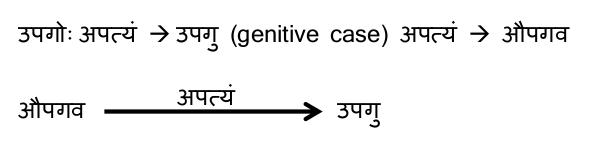
\includegraphics[width=0.8\textwidth]{Upagu}
    \caption{Relation between a Taddhita nominal and its base nominal}
    \label{upagu}
\end{figure}

\section{Objective}

Though Aṣṭādhyāyī was intended for human understanding and usage, this work attempts to automate the process of deriving Taddhitas in complete adherence to Aṣṭādhyāyī. The work aims to generate the correct form of affixation for any given nominal by following the sequence of rules applied as per Aṣṭādhyāyī in the derivation process. In this thesis, we propose an implementation model that helps in organizing the rules of Aṣṭādhyāyī, such that the organization leads to an automated triggering of rules for proper affixation of nouns. For the derivation process, Pāṇini uses a rich set of linguistic features ranging from phonetic features to semantic features. The system tries to keep record of all those features that was acquired at each step of the derivation and stores them as object attributes such that, the feature information is not lost, and hence can be used for further analysis, reusing the for other derivations and linking various relations between different nouns. This approach doubles as a pedagogy tool for the learners and enthusiasts of Sanskrit language and its grammar. Understanding of prakriya or the derivation process is very crucial in understanding of Sanskrit grammar. As the generator has potential of deriving the final form as well as the sequence of rules triggered, a new learner can understand the various transformations that occur in the process for the derivation from base to final form.
\\ \\
In ancient India, teaching has been primarily done orally, where the disciples learn from
their teacher through reciting of the sutras or rules. Aṣṭādhyāyi is no exception to it, but
due to lack of a well-documented written form, some of its information that was assumed
that a learner should possess as a prerequisite has been lost as time passed by from generations
to generations. The unavailability of those information especially related to Rule selection, conflict resolution and blocking among rules of Aṣṭādhyāyi, led to academic debates among
scholars. There has been different schools of thought, and there are different methods proposed, though there is no single method which has converged to a consensus. The proposed system 
is open to various conflict resolution techniques that have gained some ground over
the period. We will be applying various conflict resolution methods and more importantly
the schema of design allows adding many more conflict resolution techniques as per the
the programmer's choice as a pluggable module. Once a conflict resolution method is implemented, then the method's effectiveness may be validated through the results it produces and then its merits
and demerits be compared with results so obtained from other conflict resolution methods
as well.
\\ \\
The objectives of this thesis can be enumerated into the following three tasks:
\renewcommand{\labelenumi}{$\Roman{enumi}$}
\begin{enumerate}
\item Automation of Taddhita section of Aṣṭādhyāyī, so as to simulate the affixation process of derivative nouns and to evaluate how the rule organization helps to handle affix polysemy, homonymy and synonymy.

\item Implementation of various methods for rule selection, conflict resolution and blocking of rules and to check its effects in Taddhita section and in other general cases.

\item Implementation of a  model for storage of linguistic features that are obtained by the entities participating in derivation and how the same can be used for later derivations and analysis. 

\end{enumerate}

Hence the work requires to automate rules in Aṣṭādhyāyī that deal with Taddhita section as well as other associated rules, which help in the derivation process.

\section{Implementation Model}

The proposed system adopts a completely object oriented approach in modeling Aṣṭādhyāyī. The rules of Aṣṭādhyāyī are modeled as classes and so is the environment that contains the entities for derivation. The rules are then grouped based on the notion of topicality by virtue of anuvṛtti. In our proposed system the rule group formation is achieved through formation of inheritance network i.e. multilevel inheritance formed between individual rule classes, which has been inspired from the inheritance network that Pāṇini used in Aṣṭādhyāyī \cite{deo07}. Pāṇini uses anuvṛtti to carry forward the inherited components to child rules, though it needs to be noted that signifying of the inheritance is one of the aspects of anuvṛtti, and hence our proposed model does not form the inheritance network over all the usages of anuvṛtti, but rather a subset of it. The principles discussed in Aṣṭādhyāyī that enable rule selection and rule application like \textsl{ A.1.4.2} {\skt विप्रतिषेधे परं कार्यम्}, \textsl{ siddha} and \textsl{ asiddha} are built right into the core architecture of proposed system. In addition to these principles, the system provides a functionality to adopt different conflict resolution methods that are discussed outside of Aṣṭādhyāyī. The system does not restrict itself by adopting any particular conflict resolution method, instead it facilitates to try out various methods that have been mentioned in various scholarly works. This will thus help to evaluate various methods and report on their accuracy as no single set of conflict resolution methods has gained consensus among the scholars.

\section{Organization of thesis}

In Chapter \ref{sect:related}, we will be discussing about various attempts towards formalizing rules of Aṣṭādhyāyi, and modeling Aṣṭādhyāyi in part or full to a automated system. In Chapter \ref{chapter 3}, we will look into the linguistic and structural features of Taddhita section. We will be discussing about various linguistic characteristics that the affixes in the domain possess. We will also be looking into the arrangement of rules in Taddhita section and how the arrangement forms an inheritance hierarchy. In Chapter \ref{chapter 4} we will be describing the working of the proposed system, tools and techniques used for the implementation and also modeling of data environment and rule classes. The chapter will also talk about the various conflict resolution methods  for rule selection which we have employed and its effect on some of the well known instances in conflict resolution \cite{cardona65}, \cite{scharf10a}.
% Section \ref{sect:egderi} will show a step by step derivation of a nominal from another base noun..
Chapter \ref{chapter 5} will show the results of the experts evaluation we have conducted. We have also discussed the analysis of those wrong cases that the experts have observed. Finally, Chapter \ref{chapter 6} discusses the applicability of the proposed schema as a general framework to model entire Aṣṭādhyāyi by considering how the proposed system handles rules that are not specific to the derivation of a derivative noun. We also discuss the salient features and application domains of the system along with directions for future research.

\chapter{Related Work}
\lhead{Chapter 2. Related Work}
\chaptermark{Related Work}
\label{sect:related}

\section{Introduction}
Aṣṭādhyāyi has received much attention from computational linguists from the latter half of
20th century. Aṣṭādhyāyi was much lauded for its brevity, completeness and computational
insights it provides. There have been works from eminent scholars about the formalism of Pāṇini’s Grammar, its expressive power, and the derivation process (prakriyā) it follows. In Section \ref{ling} we will be discussing about the works on linguistic aspects and computational insights that Aṣṭādhyāyi provides. In Section \ref{autom} we will be looking into the various attempts in automating Aṣṭādhyāyi. The chapter will be concluded with Section \ref{concSec} discussing about the saliency and the ingenuity of the work described in this thesis how those works referred in this chapter have influenced the line of thought for thesis.

\section{Linguistic Aspects of Aṣṭādhyāyi}
\label{ling}
 Seminal works from \newcite{cardona65} and \newcite{staal65}  on formalizing rules of the grammar with stress on the meta-rules that state about the context sensitive aspects was a starting point with further enhancements from \newcite{cardona69} where he applies his formalization for more rules that is related to phonetic changes. 
\\ \\
\newcite{cardona07} highlights the relevance of affixation and how it is well integrated with syntax as a continuum in Pāṇini’s derivational system. He points out the contrast that Pāṇini’s system bears with the system that western grammarians follow, where morphology and syntax are treated as independent components in derivation. \newcite{kiparsky12} focus on the expressive power of
Aṣṭādhyāyi rules and also the expressive power of formalism that Pāṇini used to design
Aṣṭādhyāyi. They demonstrate that the formalism of the grammar has far more expressive power than that of regular languages and Context Free Languages. Their work emphasizes on the power of formalism that has built-in capacity for disambiguation at syntactic level. 
\subsection{Taddhita}
\newcite{bhate89} talks about the organization of Taddhita rules specifically and goes into detail about the domain of influence of default affixes and then the sub-domain of semantic senses inside the affix domain. The work also discusses in detail about how the Taddhita section differs from other kind of noun derivations like the kṛdanta section which is, nouns derived from verbs and also from the samāsa which is, compound words formation. \newcite{deo07} in her work coins the constrained separatism approach, which she claims what Pāṇini has followed in Taddhita. She also states idea of networks of rules that helps in the derivation process.


\section{Automation of Aṣṭādhyāyi}
\label{autom}
\newcite{hyman07} developed a finite state transducer after re-framing individual rules in Aṣṭādhyāyi, resulting in generation of strings that belong to regular languages and performs sandhi ({\skt सन्धि}) at word boundaries for any two given word combinations. Hyman had introduced an XML vocabulary for encoding rules in Aṣṭādhyāyi that helped him in implementing the finite state transducer. \newcite{scharf09c} discusses about Scharf's and Hyman's combined efforts in developing XML formalization that not only deals with sandhi but also with nominal declensions and verb conjugations. 
\\ \\
There have been various attempts to automate Aṣṭādhyāyi in parts as well as modeling it entirely.  \newcite{goyal07} implemented an inflectional morphology generator that takes as input a noun
from the user and then generates all 21 forms of noun declensions, known as \textsl{ vibhakti}
system in Sanskrit grammar. The authors talk about the programming perspectives that need to be
considered when encoding rules in Aṣṭādhyāyi, and various computational aspects that
Aṣṭādhyāyi possesses. They also talk about the need of conflict resolution methods for competing
rules that can be applied in the same context. \newcite{jha07} has developed a system that is an
inflectional morphology analyser. They have developed independent systems for verb and noun
forms and their corresponding inflections. Though their work was not related to simulating  Aṣṭādhyāyi, but they claim that they take into account the Pāṇinian way of analysis.   \newcite{kumar14} takes on generation of Sanskrit compounds called as samāsa that deals with about 400 rules of Aṣṭādhyāyi which helps them to form compound words from independent words in Sanskrit. Their work talks about various kinds of semantic features that act as the constraints governing compound formation. The Language Technologies Research Centre (LTRC) of IIIT Hyderabad has developed Dependency parsers for many Indian languages including Hindi based on the Pāṇini’s kāraka system. They have used a modified version of kāraka system of Pāṇini to capture the free-word order property that some of the Indo-European languages possess \cite{bharati2008two}.
\\ \\
\newcite{subbanna09} have talked in length about the Computational Structure of the Aṣṭādhyāyi, and introduced the concept of rules that continuously observe the environment or the subject to which modifications are to be made. They have also talked about \textsl{ Siddha, Assidhavat and Asiddha } principles used in Aṣṭādhyāyi.There has been an in-depth study on \textsl{ siddha and asiddha} principles by \newcite{joshi87}, where they talk about the order in which rules need to be applied. \newcite{subbanna09} mentioned about the grouping of rules based on the general-exception relation between rules and formation of rules as a tree structure, but commented that the feasibility of automation needs to be checked.  They also talk about various conflict resolution methods that are mentioned in the sūtras as well as in other vārttikas. \newcite{subbanna10} presented a computational model based on the principle of \textsl{ asiddhatva}, an improvised model over the one discussed in \newcite{subbanna09}. \newcite{mishra07} talks of the nature of grammar which performs the analysis of constituent elements and then its reconstitution using various set of operational rules as mentioned in Aṣṭādhyāyi. \newcite{mishra10} in his work discusses about \textsl{ vedāṅga } principles and extends his work by considering the common methodological approach of ancillary disciplines for rule application. His work provides a good walk-through for the entire derivation process that begins with introduction of atomic elements to coming up with the desired final form.  \newcite{kulkarni09} establishes the issue with phonological over-generation that can occur, if one is to strictly adhere to the rules defined by Pāṇini. \newcite{skmishra09} sheds some light in formalizing semantic categorization rules when he deals with kāraka systems. These kind of issues have been a matter of debate among linguists for quite long. Many principles that are not stated in Aṣṭādhyāyī but in other texts written at various points of time have surfaced to deal with such issues, mainly those which concern about conflict resolution in rule selection. \newcite{cardona97} discusses  about various principles like \textsl{ utsarga-apāvada}, \textsl{ antaraṅga-bahiraṅga}, \textsl{ nitya-anitya} etc. in detail.

\section{Conclusion}
\label{concSec}

To the best of the authors' knowledge, the system which we are going to propose is the first of its kind, that is focused specifically on generation of  derivative nouns. The proposed system embraces a unique approach of forming rule groups where similar rules are grouped together to form a Directed Acyclic Graph (DAG). The similarity of rules is based on the notion of topicality present among the rules by virtue of usage of anuvṛtti. The approach can be treated as analogous to the model, what is proposed in \newcite{subbanna09}, but they propose the formation of similar topic DAG through utsarga-apāvada relations. One cannot comment on the similarity of the approaches without a proper comparison of DAGs formed from both them. Moreover \newcite{subbanna09} mentioned that they had not checked the feasibility of automating their notion of rule group formation. Another important feature that our system uses is that it automatically notifies the relevant rule classes whenever the data environment state changes. This eliminates the overhead of linear searching over each rule, or each rule polling the environment to find its application. Instead the mechanism allows the rules to be updated about environment state changes whenever there is one and yet the rule classes can refrain from state dependency issues with the environment  \cite{szallies1997using}.  







%%%%%%%%END OF CHAPTER 2 %%%%%%%
 
%%%%%%%%%%%%%%%%%%%%%%%%%%%%%%
 %CHAPTER 3
%%%%%%%%%%%%%%%%%%%%%%%%%%%%%%%
\chapter{Linguistic and Structural Aspects of the Taddhita Section}
\lhead{Chapter 3. Linguistic and Structural aspects of the Taddhita Section}
\chaptermark{Linguistic and Structural aspects of the Taddhita Section}
\label{chapter 3}

In the Taddhita section, Pāṇini identifies about 300 semantic relations under which Prātipadikas can be generated with Taddhita affixes. It is mentioned as a sub-section to \textsl{ pratyayādhikāra} that deals with all kinds of affixes. The rules in Taddhita section deal with three entities namely semantic relations, affixes and stems or collection of stems from \textsl{ gaṇapāṭha}. The rules are defined in such a way so as to facilitate affixation of the proper Taddhita affix with respect to semantic relation intended. The rules often deal with properties of the entities involved at various levels from phonological, morphological, syntactic and semantic levels. There are two types of derivations possible that involve Taddhita affixes \cite{rsbook}.

\\ \\ \centerline{Prātipadika + Taddhita-affix}  \\ \centerline{Prātipadika + Taddhita-affix + strī-affix} 

\section{Linguistic Phenomena in Derivational Morphology}

Derivational morphology in Sanskrit, like in many other languages poses some of the well
known facts about many to many correspondences between forms and affixes. Taddhita affixes exhibit affix polysemy, homonymy, synonymy and non-compositionality. Considering a single affix and multiple senses we can discuss about affix polysemy and homonymy and with multiple affix and same semantic relation we can talk about affix synonymy. In fact, in Sanskrit non-compositionality of the taddhita affixes are also well discussed . In affix polysemy, the same affix is used to denote related senses like in the case of patronymic and provenance relation. In affix homonymy the same affix is used in distinct and unrelated semantic contexts like in the case of personal nouns or abstract nouns. Affix synonymy deals with the same semantic sense but
uses different affixes. For example, for the  patronymic relation {\skt अपत्यम्}, multiple affixes can be used, like {\skt अ(ण्), अयन(फक्), इ(ञ्)} depending on the stems used \cite{deo07}. Table  \ref{PHSH}, Table \ref{PHSP}, Table \ref{PHSS}  show some instances of each of these phenomena, with analogy to the same phenomena in English language.
\\
% Please add the following required packages to your document preamble:
% 

\begin{table}[h]
\centering
\caption{Affix Polysemy in Sanskrit and English}
\label{PHSP}
\begin{tabular}{|c|l|l|l|}
\hline
\multicolumn{4}{|c|}{Affix Polysemy}                                                                                 \\ \hline
\multicolumn{2}{|c|}{Sanskrit (affix - {\skt अ})}                & \multicolumn{2}{c|}{English (affix -ian)}                \\ \hline
Base                       & \multicolumn{1}{c|}{Derived} & \multicolumn{1}{c|}{Base} & \multicolumn{1}{c|}{Derived} \\ \hline
\multicolumn{1}{|l|}{\skt मथुर} & {\skt माथुरा}                       & India                     & Indian                       \\ \hline
\multicolumn{1}{|l|}{\skt उपगु} & {\skt औपगव}                         & Orwell                    & Orwellian                    \\ \hline
\end{tabular}
\end{table}
\\
\begin{table}[h]
\centering
\caption{Affix Homonymy is Sanskrit and English}
\label{PHSH}
\begin{tabular}{|c|l|l|l|}
\hline
\multicolumn{4}{|c|}{Affix Homonymy}                                                                                  \\ \hline
\multicolumn{2}{|c|}{Sanskrit (affix - {\skt अ})}                 & \multicolumn{2}{c|}{English (affix -ian)}                \\ \hline
Base                        & \multicolumn{1}{c|}{Derived} & \multicolumn{1}{c|}{Base} & \multicolumn{1}{c|}{Derived} \\ \hline
\multicolumn{1}{|l|}{\skt निपुण} & {\skt नैपुण}                        & Library                   & Librarian                    \\ \hline
\multicolumn{1}{|l|}{\skt शुक}   & {\skt शौका}                         & Comedy                    & Comedian                    \\ \hline
\end{tabular}
\end{table}

\\
\begin{table}[h]
\centering
\caption{Affix Synonymy in Sanskrit and English}
\label{PHSS}
\begin{tabular}{|c|l|l|l|l|l|}
\hline
\multicolumn{6}{|c|}{Affix Synonymy}                                                                                                   \\ \hline
\multicolumn{3}{|c|}{Sanskrit (Patronymic)}                                             & \multicolumn{3}{c|}{English (Provenance)}    \\ \hline
Base                        & \multicolumn{1}{c|}{Derived} & \multicolumn{1}{c|}{Affix} & \multicolumn{1}{c|}{Base} & Derived  & Affix \\ \hline
\multicolumn{1}{|l|}{\skt उपगु}  & {\skt औपगव}                         & {\skt अ}                          & India                     & Indian   & -ian  \\ \hline
\multicolumn{1}{|l|}{\skt अश्वल} & {\skt आश्वलायन }                    & {\skt आयन }                        & Kerala                    & Keralite & -ite  \\ \hline
\end{tabular}
\end{table}

\section{Organization of Taddhita Rules}
\label{orgTad}
Taddhita section is primarily subdivided into five \textsl{ pratyayādhikāras} or domain of control
of five affixes.
\renewcommand{\labelitemi}{$\blacksquare$}
\begin{itemize}
  \item The five rules are:
\renewcommand{\labelenumi}{$\Roman{enumi}$}
\begin{enumerate}


  \item \textsl{ A.4.1.83} {\skt प्राक् दीव्यतः अण् } - {\skt अण् } suffix is the default affix to be used for affixation for all the rules till \textsl{ A.4.4.1}. The influence of \textsl{ A.4.1.83} is till the term {\skt दीव्यति} is found (or till another pratyayādhikāra is found) and {\skt दीव्यति} appears in rule \textsl{ A.4.4.2} {\skt  तेन दीव्यति खनति जयति जितम्}. 
  \item \textsl{ A.4.4.1} {\skt  प्राक् वहतेः ठक् । } - {\skt ठक् } suffix is the default affix to be used for affixation for all the rules till \textsl{ A.4.4.76}. {\skt  वहति} appears in rule \textsl{ A.4.4.76} {\skt तत् वहति रथयुगप्रासङ्गम्}.
  \item \textsl{ 4.4.75} {\skt प्राक् हितात् यत् } - {\skt यत् } is the default affix to be used for affixation for all the rules till \textsl{ A.5.1.5}.{\skt हितम्} appears in rule \textsl{ 5.1.5} {\skt  तस्मै हितम्}. 
  \item \textsl{ 5.1.1} {\skt  प्राक् क्रीतात् छः } - {\skt छः } is the default affix to be used for affixation for all the rules till \textsl{ A.5.1.37 }{\skt  क्रीतम्} appears in  rule \textsl{ 5.1.37} {\skt तेन क्रीतम्}.
  \item \textsl{ 5.1.18} {\skt प्राग् वतेः ठञ् } - {\skt ठञ् }is the default affix to be used for affixation for all the rules till \textsl{ A.5.1.115}. {\skt वतिः} appears in rule \textsl{ 5.1.115} {\skt  तेन तुल्यं क्रिया चेत् वतिः }. 
  
\end{enumerate}
\end{itemize}

\begin{figure}[h]
    \centering
	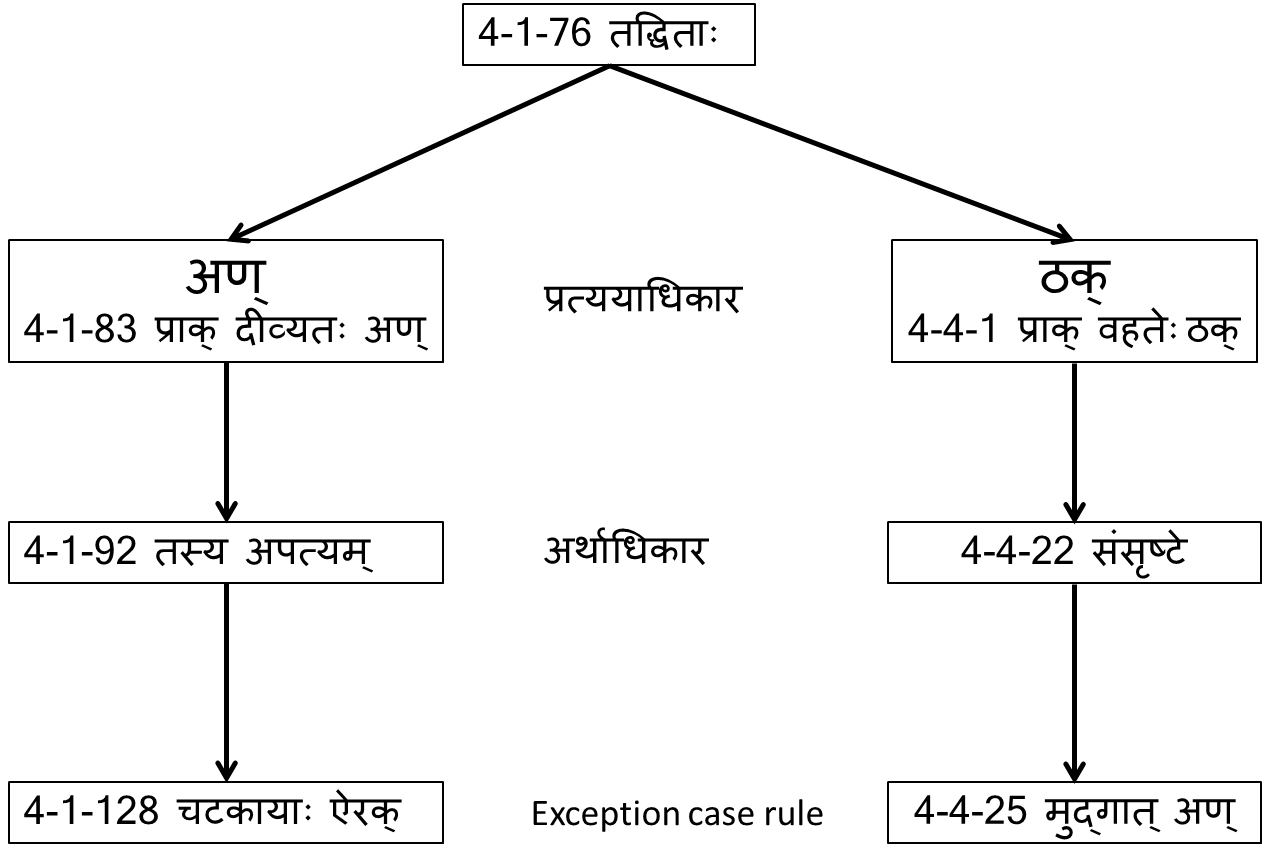
\includegraphics[width=0.8\textwidth]{tad}
    \caption{An instance of inheritance hierarchy in Taddhita section}
    \label{fig:inheritance}
\end{figure}


Now each of the above given rules, which can be called as the pratyayādhikāra rules, specifies what is the most prominent affix or the default case affix that can be applied to all the rules which are under its domain. For the set of rules under a single pratyayādhikāra, they are further categorized on the basis of arthādhikāra rules. Each arthādhikāra heads a set of rules which are a proper subset of rules that come under the pratyayādhikāra. The arthādhikāra rules state the semantic conditions or the semantic rules under which the default affix can be attached. Arthādhikāra rules serve the purpose of a topic head that groups a set of rules as a rule group based on a topic, which is a semantic relation here and it also acts as an operational rule ({\skt विधि}), as it carries the semantic sense under which the affix can be attached. Rules \textsl{ A.4.1.92} {\skt तस्य अपत्यम्}, \textsl{ A.4.2.1} {\skt तेन रक्तं रागात्}, \textsl{ A.4.2.69} {\skt तस्य निवासः} etc. denote the semantic senses such as patronymic, coloured by means of that and provenance respectively. This kind of arrangement handles affix polysemy and affix homonymy. But to handle affix synonymy, there are other operational rules, that come under the domain of arthādhikāra rules. They can be seen as exception rules or rules to handle special cases. These rules limit the application of default affix specified in pratyayādhikāra and mention what other affixes can be used instead, under special conditions. In this way, affix synonymy and non-compositionality is taken care of.\\ 
\newcite{deo07} calls this form of arrangement as constrained seperationism, where the rules form a multilevel single inheritance network. The template for the multilevel inheritance network will be of the type,  "Default Affix rule" -"Semantic Sense rule" - "Special case rules". Figure \ref{fig:inheritance} shows an instance of how the hierarchy in Taddhita works. As already discussed, \textsl{ A.4.1.83} states about the default affix {\skt अण्} for rules under its domain, \textsl{ A.4.1.92 }states about the patronymic relation under which a nominal will get the default affix. Now rule \textsl{ A.4.1.128} states about a special case when the stem {\skt चटका} is used with the patronymic relation. In such a case the suffix {\skt ऐरक्} needs to be attached. This rule overrides the default case rule. Now consider rule \textsl{ A.4.4.25.} This rule talks about usage of {\skt अण्} as an exception or special case when a stem {\skt मुद्ग} is used. The rule has \textsl{ A.4.4.1} as its default affix rule and the default affix for the domain is {\skt ठक्}. The rule's semantic sense is {\skt संसृष्टे}, which means 'properly mixed with'. Here the rule \textsl{ A.4.4.25} accounts for the non-compositionality of the affix {\skt अण्} and is not specified in its domain but as an exception rule in another default affix domain. In this way Pāṇini is able to achieve constrained separationism \cite{deo07} which is an alternative to both the separationist and non-separationist viewpoints in the case of derivational morphology. Here Pāṇini has employed a multilevel but single inheritance hierarchy through pratyayadhikāra and arhtadhikāra, where arthadhikāra inherits from only one pratyaya, and affix synonymy that may occur is being handled through exception handling rules.
\\ \\
It is to be noted that there are some more rules in the Taddhita section which do not come under any of the five pratyayadhikāra rules. Those rules have arthādhikāras of their own but has no default affix to be attached. This group of rules is treated as extraneous to otherwise systematic network of the section \cite{bhate89}. As we will be discussing about the implementation schema of proposed generation system in the subsequent section, it will become evident that this anomaly in no way is going to affect the system.


\section{Techniques of Rule Arrangement in Taddhita and Aṣṭādhyāyi}

Aṣṭādhyāyi is a linear arrangement rules across eight chapters as mentioned. Aṣṭādhyāyi
was supposed to be passed on in oral form. So Pāṇini had to take care of two aspects. He
needed to somehow define thematic domain and the boundary of the domain for the
rules, and also he needs to achieve brevity as he needed to keep the entire Aṣṭādhyāyi as
short as possible for ease of recitation. He has used special kind of rules called adhikāra rules
for specifying thematic domain and further sub-domains for a given set of rules. He has
efficiently used the concept of ellipsis in the form of anuvṛtti to achieve brevity

\subsection{anuvṛtti}

\begin{figure}[h]
    \centering
	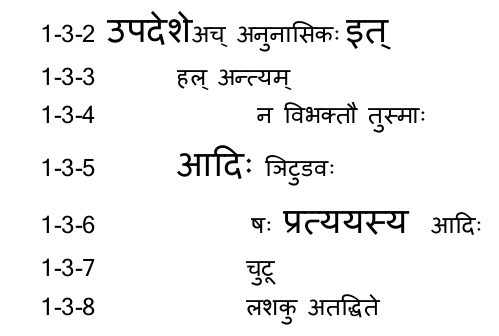
\includegraphics[width=0.8\textwidth]{anuIn}
    \caption{anuvṛtti of 'it' section in Aṣṭādhyāyī}
    \label{fig:anuFig}
\end{figure}

In anuvṛtti or what we can call as recurrence, in order to keep the individual sutras short,
some information is omitted from those sūtras which can be obtained from subsequent
rules. So a rule when read alone doesn’t provide the complete information and hence
needs to be read with the entire anuvṛtti. For eg the rule number \textsl{ A.4.1.123} is {\skt शुभ्रादिभ्यः च} which means "for stems in śubra and co. as well”, and does not makes any sense if not provided with any other information.  But the same rule when read with anuvṛtti will be {\skt शुभ्रादिभ्यः च प्रत्ययः परः च आद्युदात्तः च तद्धिताः समर्थानां प्रथमात् वा प्राक् दीव्यतः अण् स्त्रीपुंसाभ्यां नञ्स्नञौ भवनात् तस्य अपत्यम् ढक् }. Here the rule translates to "for stems in śubhra and co. as well, that come under adhikāra of
pratyaya, under the sub domain of taddhita, and pratyayādhikāra of aṇ where the semantic relation is apatyam and if the stem is in genitive, apply the pratyaya ḍhak. ” anuvṛtti may be passing down of
entire rule as in \textsl{ A.4.1.82} or a partial component inheritance as in case of \textsl{ A.4.1.120}. The components being passed down as anuvṛtti can be a semantic relation, a condition to be
satisified, a context in which it needs to be applied, an adhikāra or a particular operation. anuvṛtti or recurrence can be seen as block of control as well. To visualize consider the
snippet given below in Figure \ref{fig:anuFig}. Here anuvṛtti is denoted via indentation and those which are inherited is made bigger in size.

\subsection{Adhikāra}
It is a form of inheritance where classes of rules belonging to same thematic domain
inherit thematic head so as to be grouped together \cite{deo07}. The pratyayadhikāra \textsl{    A.4.1.83} is one such adhikāra rule. The rule infact is a sub-domain inside \textsl{ A.4.1.76}, which is a subdomain of \textsl{ A.3.3.1}. Similarly rule \textsl{ A.4.4.1} share common ancestor adhikāra rules as of that for \textsl{ A.4.1.83}. Hence we claim that the Aṣṭādhyāyī is a multilevel inheritance hierarchy. The device of adhikāra indicates the homogeneity of topic \cite{joshi1984fundamentals}. It classifies the rules that come in its domain with rules that come in a different domain. A rule can never be under the influence of two adhikāra rules where one adhikāra is not a subset of the other in terms of domain reach. A rule can have multiple adhikāra as shown in that for \textsl{ A.4.1.92}, it has adhikāra rules starting from \textsl{ A.4.1.76}. But no two adhikāra rules are at equal level, each adhikāra rule is a subset of other rule. Hence there can be multilevel inheritance but no multiple inheritance in Aṣṭādhyāyī.

%%%%%%%%END OF CHAPTER 3 %%%%%%%
 
%%%%%%%%%%%%%%%%%%%%%%%%%%%%%%
 %CHAPTER 4
%%%%%%%%%%%%%%%%%%%%%%%%%%%%%%%
\chapter{System Implementation and the Derivation Process}
\lhead{System Implementation and the Derivation Process}
\chaptermark{System Implementation and the Derivation Process}
\label{chapter 4}


\section{Overview of the Implementation System }
\label{sect:impl}

For automating the derivation process, we suggest the following method which is based on object oriented concepts. The derivation process happens in a central object called as environment, which essentially has methods and attributes that takes care of conversion of user input to suitable data structures, triggering of rules and book-keeping of rules applied. Each rule forms a class and each instance of the rule class (henceforth to be referenced as rule itself) is registered with the environment, such that whenever there is a change in the environment, the rules are notified. Each rule checks for the possibility of it being applied on the environment and for a rule, if all its conditions are satisfied, ideally the rule can be applied on the environment. However, in a general scenario  multiple rules may claim their competency for application on the environment. To handle such scenarios we keep those competing rules in a list called candidate list. Then a conflict resolution method is employed which decides the winner rule. The winner rule gets to apply on the environment and other rules are removed from list. By removal of rules other than the winner rule, we mean that the removed ones are not applied on the present instance of environment, although they are notified when the environment change happens again. Figure \ref{fig:impl-fig} shows the schema of the implementation system.
\\
\begin{figure}[h]
    \centering
	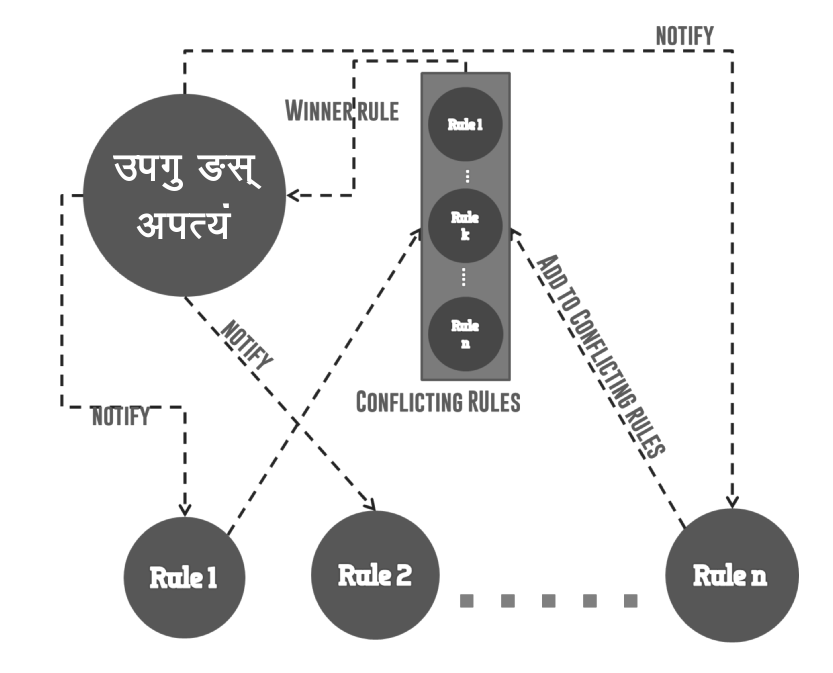
\includegraphics[width=\textwidth]{impl}
    \caption{Overview of Implementation System}
    \label{fig:impl-fig}
\end{figure}
\\ \\
As it is evident from discussion about Taddhita section, Pāṇini among various applications of anuvṛtti, uses it for carrying the topicality between different rules as well. It is to be noted that adhikāra rules are rules whose sole purpose is mentioning the topicality of the rules under its domain of influence. But even for adhikāra rules, anuvṛtti itself is used for carrying the domain's influence to other rules. Apart from the adhikāra rules, there are other rules as well in which anuvṛtti is used to carry the topicality. For example consider the rules concerning {\skt  इत्}, i.e. rules from 1.3.2 to 1.3.8. Here {\skt उपदेशे and इत्} are being carried forward to other rules as well. {\skt उपदेशे}, which means 'when an upadeśa is encountered', perform some action. This condition leads to a common topicality for all the rules under the anuvṛtti. This is similar to the notion of arthādhikāra rules in Taddhita where the notion of semantic sense is being carried forward to subsequent rules through anuvṛtti. Both the techniques, anuvṛtti and adhikāra are employed in the entire Aṣṭādhyāyī and are not unique to the Taddhita section. We can infer that a subset of the anuvṛtti rules, mostly the ones which carry the notion of topicality can be used to design an inheritance hierarchy of classes.  For the  implementation we will be using this notion of topicality via anuvṛtti, in grouping of rules to form rule groups which is an inheritance hierarchy among rules and the rule in which the portion of anuvṛtti appears, becomes the head rule.
\\
\subsection{Tools and Techniques Used}
\label{sect:tools}
We are following a completely object oriented approach for the implementation of the system.
The following tools and techniques will be employed to achieve the principles discussed in section \ref{sect:impl} 

\\
\subsubsection{Observer Design Patern}
Observer design pattern defines a one-to-many dependency between objects so that when one object changes state, all its dependents are notified and updated automatically \cite{obs}. The object to which the state changes occur is called subject and it maintains a list of its dependents, called observers. As shown in Figure \ref{fig:obsUML}, each observer object which is the sūtra or rule in our case, is registered to an object called as “Subject” class which represents the environment in our case. Subject class has a method to register the observers. Whenever a change in value of some attribute of subject occurs, it calls the method 'notify' of observer abstract class, which is implemented for each object of the Observer.

\begin{figure}[h]
    \centering
	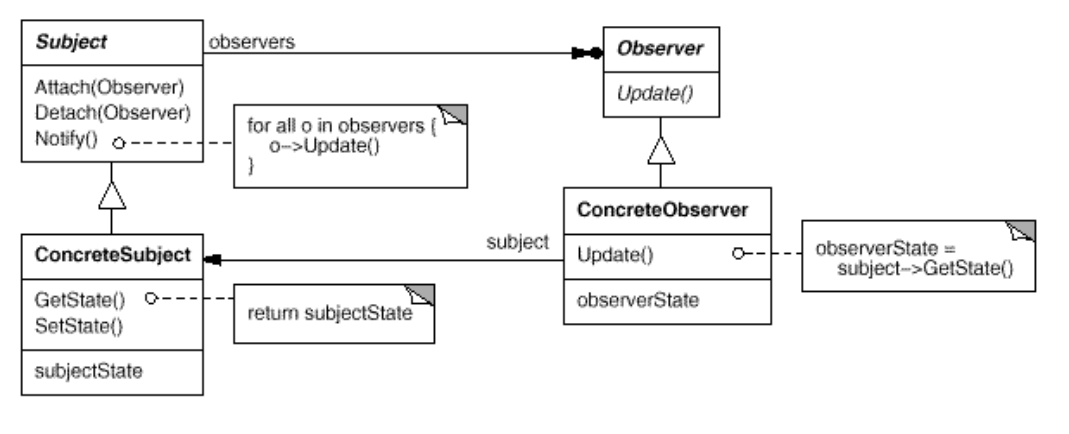
\includegraphics[width=\textwidth]{obsUML}
    \caption[UML diagram for observer design pattern]{UML diagram for observer design pattern.\cite{obs} }
    \label{fig:obsUML}
\end{figure}

\\
\subsubsection{Multilevel Inheritance}

To form rule groups i.e. inheritance network among rules we use multilevel inheritance between the rules. Though multilevel inheritance is allowed, multiple inheritance is not allowed in the system and hence no single rule will inherit from two distinct rules directly. Figure \ref{fig:UMLinher}
shows the inheritance achieved for each class in Aṣṭādhyāyī. All classes inherit from a base class
called "sūtra", which is a generic class that defines all possible features that a rule or sūtra can possess. All other rules inherit from it. The adhikāra rules, anuvṛtti of interpretive rules, default condition rules etc. form super class for other operational rule classes. 

\begin{figure}[h]
    \centering
	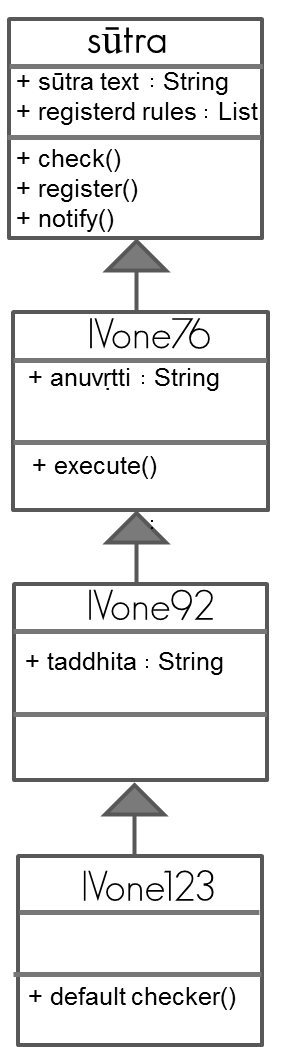
\includegraphics[width=0.2\textwidth]{UMLinher}
    \caption{UML diagram for multilevel inheritance}
    \label{fig:UMLinher}
\end{figure}


\\
\subsection{Rule Triggering and Propagation}
The environment forms the subject class for the observer design pattern. However, not all rules are
observing the environment but only those rules that do not come under the domain of any adhikāra rules or a controlling head of a rule group through anuvṛtti (which are mostly rules that assigns the technical terms to assignments). Those are represented by classes R1, R2 and so on in Figure \ref{fig:fullImp}. Then there are rule groups as represented by RG1, RG2 and so on. These are collections of rules with same head. The rule classes that come under the same head in the group, inherit from the head rule class. The head rule object, as per observer design pattern registers the inherited classes' objects as observers. Now the head class notifies the observers whenever the environment satisfies the head rule's conditions. The conditions checked are those conditions that need to be satisfied by all the rules registered under the head.  Here, by 'head', we mean either an adhikāra or a component passed on by anuvṛtti. Now top level rules are those rules which observe the environment directly and get notified whenever the environment changes. For a rule, if the environment satisfies its conditions, it will be added to the candidate list. But if the environment satisfies the conditions that is applicable to an entire rule group, then the environment object is passed on to the next level and this continues till an exception or specific rule is encountered or else returns back to where the default rule resides. By this model, we can employ conflict resolution at each level, and resolve some of them locally and only rules that have no common head at any level come to the candidate list at top-most level, from where the winner rule will be selected.
\\ \\
Once a winner rule is selected, the rule's intended action is executed first and then its parent object is called which performs its relevant portion in execution, if any. This continues until all the rules in hierarchy are called. It is to be noted that many a times certain rules like the adhikāra rules do not have anything to execute of their own, in such cases the rule object just passes on the environment to its parent object. By this design, redundancy of hard coding the same rules again and again per rule object is saved, just like the way anuvṛtti helps a person to avoid repeating the rules when reciting Aṣṭādhyāyī.

\begin{figure}[h]
    \centering
	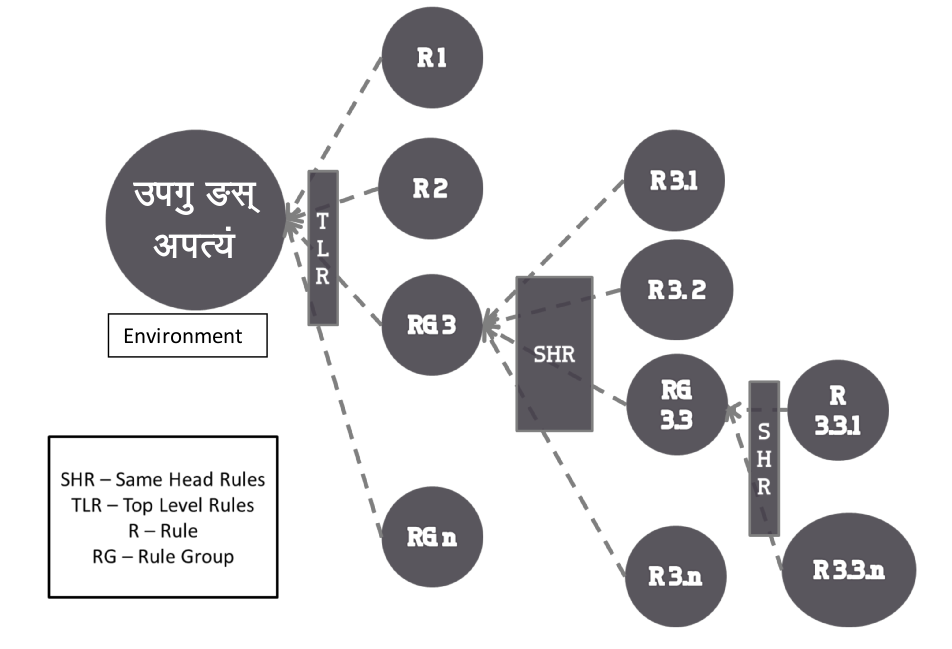
\includegraphics[width=\textwidth]{fullImp}
    \caption{ Triggering schema.}
    \label{fig:fullImp}
\end{figure}


\\
\subsubsection{Working}
\label{sect:woring}
Let us consider the working of the system with reference to affixation for semantic relation {\skt अपत्यम्}, i.e. the patronymic relation. Figure \ref{fig:tadrule} shows the trace for the affixation process of Taddhita affix when the semantic relation is patronymic and the stem is {\skt चटका}. In Figure \ref{fig:tadrule}, the solid lines show inheritance hierarchy between the rule classes. The dashed line on the left of each block shows traversing of the hierarchy by triggering of rules from head to specific rules. The traversal checks for eligible rule to apply on environment within the rule group, and this can be called as the checking phase. The dotted lines on the right of each block show the trace of rules that get executed. The starting node, i.e. the node that heads the dotted edge with label 1 is the exact rule that gets executed and other nodes in the path show those rules that have been executed due to anuvrtti. This can be called as the execution phase. As an example let us consider the case where the environment is initialized with {\skt चटकायाः अपत्यम्}.  The triggering starts from head rule at the top level i.e. from  \textsl{ A.3.1.1} to rule  \textsl{ A.4.1.128} as shown in Figure \ref{fig:obsUML}. Here in rule \textsl{ A.3.1.1}, it does not have any condition to check, so it directly notifies all of its direct descendants. Now among the direct descendants, rule \textsl{ A.4.1.1} checks for presence of any of the two affixes {\skt ङि, आप्} or if the environment has a prātipadika in it, i.e. it checks for conditions mentioned directly in the rule. As it is a prātipadika, the condition will evaluate to 'true',and all its descendants are notified. In due course, \textsl{ A.4.1.76}, \textsl{ A.4.1.83} are also notified. These rules as well do not have any extra checks as they are adhikāra rules and hence all its direct descendants are notified. When \textsl{ A.4.1.92} is notified, it checks for semantic condition and the checking turns out to be true for \textsl{ A.4.1.92}, while the checking will evaluate to 'false' for all of its sister nodes, i.e. other direct descendants of \textsl{ A.4.1.83}. The special case rules registered under \textsl{ A.4.1.92} are notified, of which \textsl{ A.4.1.128} satisfies the remaining conditions. As it does not have any rules registered to it, it becomes the terminal node and hence it is added to the candidate list. Since for this case no other rule is contesting, the rule emerges winner and starts its execution from \textsl{ A.4.1.128.} The rule adds the affix {\skt ऐरक्} to environment, and passes the environment to its parent class i.e. \textsl{ A.4.1.92}. \textsl{ A.4.1.92} does not have anything to execute of its own, so it simply passes environment to \textsl{ A.4.1.83}, which checks if any affix is already attached, as the affix '{\skt ऐरक्}' is attached in this case, no action is performed. The environment gets passed to parent node of each rule finally this terminates at top level rule \textsl{ A.3.1.1}. Now consider the derivation of {\skt उपगोः अपत्यं}. As with the case of {\skt चटकायाः अपत्यं}, the path of the rules checked for eligibility of rule application remains the same till rule \textsl{ A.4.1.92} is reached. Once \textsl{ A.4.1.92} is reached it will notify all of its descendants as well. But since no rule will find its application, \textsl{ A.4.1.92} will become the final node of the path here. It is added to candidate list, which while executing will simply call the parent rule \textsl{ A.4.1.83}. \textsl{ A.4.1.83} checks for presence of any new Taddhita affix in the environment. If the check evaluates to false, i.e. if no new Taddhita affix is found, \textsl{ A.4.1.83} treats this as default case scenario and attaches {\skt अण्}, the default case affix to environment. After each execution of a rule, the system checks for presence of any new assignment of 'technical term' or else all rules in the top level are notified as discussed in Section \ref{sect:intro-deri}.


\\
The arthādhikāra rules inherit from its corresponding pratyayādhikāra rules, apart from the ones already mentioned in Section \ref{orgTad}. When it comes to affixation, during the checking for eligibility of a rule to apply i.e at the checking phase, we need to traverse the  pratyayādhikāra rule, before an arthādhikāra rule is reached. Though a pratyayādhikāra rule is visited during checking, no action is taken there. The pratyayādhikāra rule simply passes the environment to all arthādhikāra rules which are its direct descendants. In fact for a single affixation, all the pratyayādhikāra rules get notified from its parent rule, and those rules in turn notify all their direct descendants as there is not enough information to select a single pratyayādhikāra at during the checking phase. So in effect, the process of affixation for taddhita starts by checking for the right semantic condition i.e at the arthādhikāra rules as it is in the case of traditional system of derivation. Before that, the other rules either simply pass on the environment to their descendants or check for conditions that is necessary for the process to qualify as a case for affixation under taddhita. The effect of pratyayādhikāra rule comes during the execution phase i.e at the applying of affix phase and not on the checking phase. During the execution phase the pratyayādhikāra which is parent to the winner arthādhikāra rule acts as the final gate that makes sure that the environment has the valid taddhita affix added to the environment before it reaches its parent. The rule checks if any taddhita affix is introduced by virtue of special case rules, and if no such execution has taken place, then the default affix is added to the environment. The environment is then passed on to higher level rules that takes care of other generic aspects about the environment.

     
\begin{figure}[h] 
    \centering
	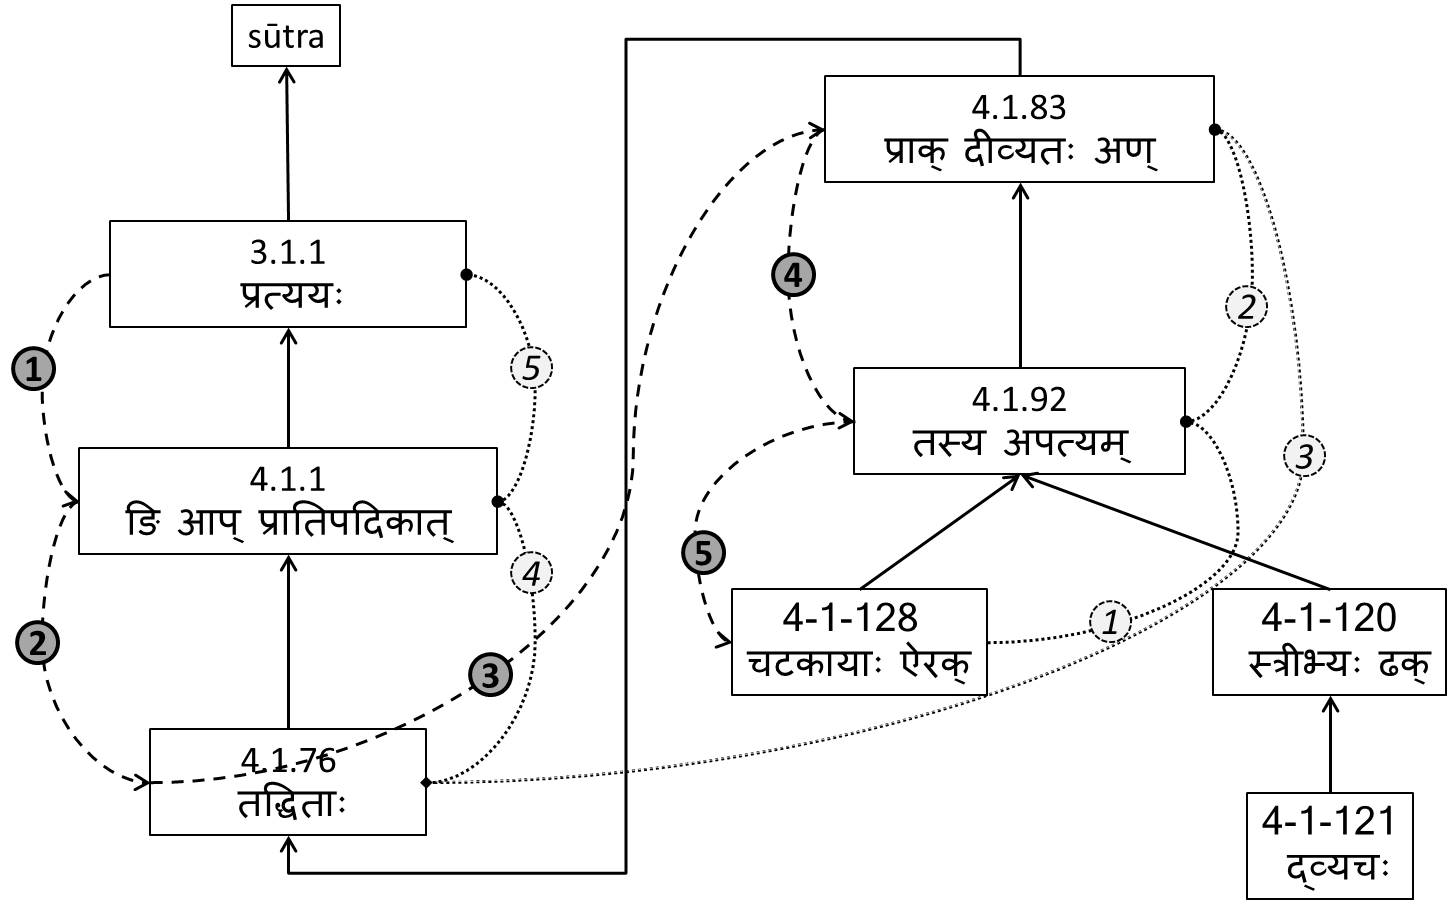
\includegraphics[width=\textwidth]{tadrule2}
    \caption{Affixation under patronymic relation for {\skt चटका}}
    \label{fig:tadrule}
\end{figure}
  
  
  
  
\\
\subsection{ \uppercase{ś}abdarūpa Representation}
The environment is an object which contains methods for navigating through top level rules, list of applied rules and the śabdarūpa object as its attribute. \uppercase{ś}abdarūpa object holds the data entities which take part in the derivation process. Entities can be stems, affixes, augments, characters or any of their properties. The most basic and atomic entity in the śabdarūpa object is another object called 'śabda'. The śabdarūpa object also contains various instances of the class 'śabda collection' , which contains a sequence of references to śabda objects along with a set of attributes that belongs to the collection. \uppercase{ś}abdarūpa object is an instance of 'śabda collection' class.  Instances of 'śabda collection' are used to represent various technical terms that may be attributed to environment or a part of it. Figure \ref{fig:enc} shows how the śabdarūpa object is set up.  Figure \ref{fig:enc} shows the śabdarūpa object after the affixation of Taddhita affix {\skt अण् }. As already seen in Section \ref{sect:woring}, the Taddhita affixation happened due to presence of technical term prātipadika. Now the technical term prātipadika is modeled as an attribute of the śabdarūpa object, and it is an object itself of the class 'śabda collection'. It contains references to sequence of all the śabda objects, which is collectively eligible for the technical term prātipadika. Similarly inside 'pratyaya' object, it has an attribute 'it marker' which also is an object  of 'śabda collection' class called 'it'. If you notice though the \textsl{ it} ({\skt इत्}) marker is {\skt ण् in अण्}, it is not the śabda's property that it is an \textsl{ it} marker. It is the property of pratyaya that gives the śabda {\skt ण्}, the property of \textsl{ it marker}. This notion is captured very well in the system. It is essential that we store them as attributes separately for further reference and usage in the derivation process. For example, consider the derivation process for āśvalāyana. The term āśvalāyana is formed from aśvala by affixing 'phak' pratyaya. Here the 'it' marker is 'k', which will be stored in 'it marker' object, and later it will be elided, and hence be removed from the 'text value' of pratyaya object by application of rules \textsl{ A.1.3.3 and A.1.3.9} . In due course of derivation the pratyaya object will get a substitution of 'āyana' for the remaining 'pha' by rule \textsl{ A.7.1.2}. Now in order to complete the derivation process, rule \textsl{ A.7.2.118} should stand valid in one of the subsequent steps. Rule\textsl{ A.7.2.118} requires a Taddhita affix with k as 'it' marker. If we had not stored this information as a separate attribute earlier, we would have lost this information and derivation would not have completed. Apart from the attributes, the śabdarūpa object has methods that performs the five operations of placement, augmentation, substitution, deletion and modification  as categorized by \newcite{rsbook} for operational rules.

\renewcommand{\labelenumi}{$\Roman{enumi}$}
\begin{enumerate}
\item Placement of a new entity - A new entity like affixation where a new independent entity is introduced to the śabdarūpa object. \textsl{ 4-1-128 { \skt चटकायाः ऐरक्}} does a placement operation. 
\item Augment an existing entity - Adding a new augment to any of the existing entities. \textsl{ A.4-1-97 {\skt सुधातुः अकङ् च }} is one such rule that performs augmentation of {\skt अकङ्} followed by a placement operation. 
\item Substitution - Replace contents of an entity or a portion of it with new substituent contents. \textsl{ A.6-1-77{\skt  इको यण् अचि}} does a replacement operation. 
\item Deletion - Remove an entity or a portion of it. \textsl{ 4-1-133 {\skt ढकि लोपः}} is a rule that performs the operation.
\end{enumerate}
Modification is performed as the combination of any of the four operations after executing the modifying action like the vṛddhi operation.
\\
     In case of \textsl{ asiddhavat} rules as discussed in \newcite{subbanna09}, the śabdarūpa object makes a complete copy of itself, one object is used for checking the conditions while in the other object, all the operations are applied. Once the system returns back to siddha section, the copy used for checking the conditions is discarded. It is also to be noted that in the representation the space between entities are also śabda objects, representing the virāma ({\skt विराम}) as per the rule \textsl{ A.1.4.110} {\skt विरामः अवसानम्}.



\begin{figure}[h]
    \centering
	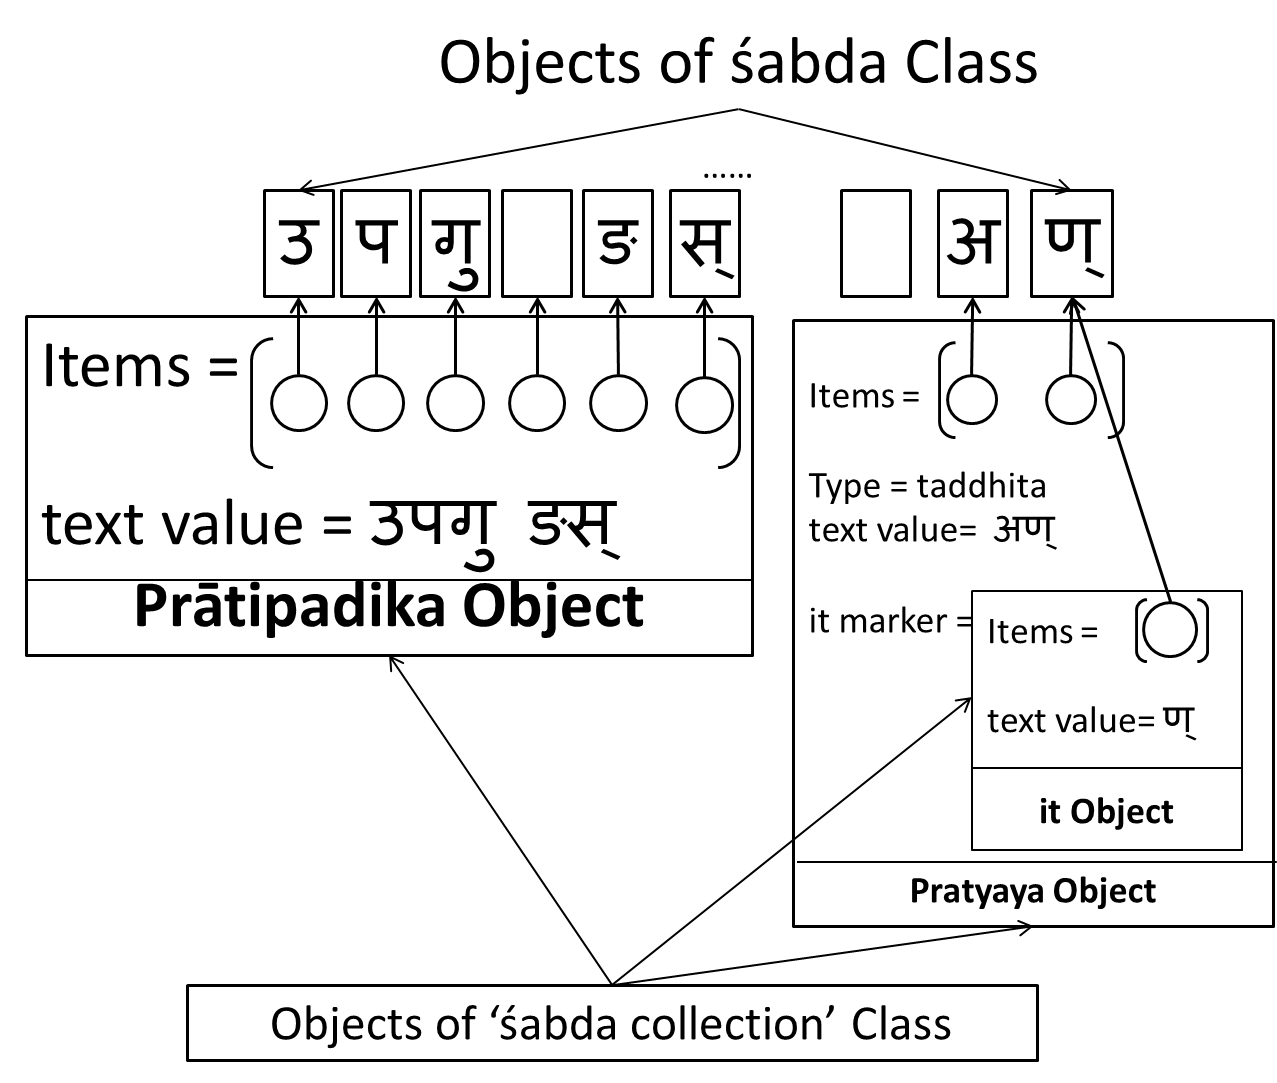
\includegraphics[width=0.8\textwidth]{environment}
    \caption{Representation of Environment object}
    \label{fig:enc}
\end{figure}

\\
\section{Derivational Process along with the storage and propagation of linguistic features.}
\label{sect:intro-deri}

In order to discuss about the derivation process or ({\skt प्रक्रिया}) of a derivative noun, let us take the derivation of derivative noun {\skt औपगव} from the nominal {\skt उपगु  }, which can be considered as the 	"Hello world" in Taddhita section. The essential steps in the derivation process are shown in Table \ref{derivation-table}.  {\skt औपगव} which means son of upagu, comes from the semantic sense {\skt अपत्यं} by the rule 4.1.92 {\skt तस्य अपत्यम्}, and the correct Taddhita affix {\skt अण् } is introduced to the environment. Once the Taddhita affix is introduced, what remains is a series of operations on the environment that results in a final form. The rules so triggered may be seen as a continuous iteration of two sub-processes. One is identification and assignment of technical terms ({\skt संज्ञा}) to the environment string or to a relevant substring of it. By this, the environment does not get modified but gains the technical term as an attribute. The interpretive rules or rules assign the technical terms to the environment and those rules are shown in the first column of Table \ref{derivation-table}. Now, by virtue of these attributes, the environment gets modified through operational rules that come within the domain of attributes as shown in the third column of Table \ref{derivation-table}.  The effect of the rule on the environment can be seen in the second column.  Triggering of operational rules is the second sub-process in the iteration and the derivation process stops when no more attributes can be attributed to the environment. Ideally, by that time the desired form must be derived. 
\\ \\
For the proper derivation of the derivational noun, it needs to attain certain technical terms as its properties, and by virtue of these technical terms, more rules will get triggered. the same technical might be used in multiple occasions or some might not be used immediately. There are cases where these properties are often needed to be preserved as these properties might be required to derive new nouns from the current noun. One such case is discussed in Section \ref{wrongCases}. Apart from technical terms, we also keep other rich linguistic features such as the intended semantic sense which will not be evident in the final word form of the new noun. Such properties can be later used to maintain relations between different nouns and label the edges of those relations.

\begin{table}[h]
\caption[Derivation Process for { \skt औपगव }]{\label{derivation-table} Derivation Process for { \skt औपगव }. Here each horizontal line partition represents one step in the derivation, where one of the operations among insertion, elision or substitution takes place in column 2. Column 1 shows assignment of some technical term, and column 3 shows subsequent operation after gaining the technical term as a property. Column 2 shows the effect due to the operation. In column 2 we can see the effect of the rules on the environment, where an insertion, elision or substitution takes place.  }

\begin{center}
\resizebox{\textwidth}{!} {
\renewcommand{\arraystretch}{1.5}
\begin{tabular}{|l|c|r|}
\hline \bf Interpretational terms to be assigned & \bf Derivation environment & \bf Operation rule to be applied \\ \hline
 & {\skt उपगोः अपत्यं} &  \\ \hline
 & { \skt उपगु ङस् अपत्यं } & \\ \hline
  { \skt तद्धित } (4.1.76 {\skt तद्धिताः}) & & \\ & & 4.1.92 {\skt तस्य अपत्यम् } \\
& {\skt उपगु ङस् अण्} & \\ \hline 
{\skt इत् } (1.3.3 { \skt हलन्त्यम्}) & & \\
& &  1.3.9 { \skt तस्य लोपः}  \\
& { \skt उपगु ङस् अ} &   \\ \hline

{\skt प्रातिपदिकम् } (1.2.46 { \skt कृत्तद्धितसमासाः च}) &  &  \\

&  & 2.4.71  { \skt सुपः धातुप्रातिपदिकयोः }  \\
&  { \skt उपगु अ } &  \\ \hline
{ \skt अङ्गम् } ( 1.4.13 { \skt यस्मात् प्रत्ययविधिः तदादि प्रत्यये अङ्गम् } ) & &  \\
&  & 7.2.117 { \skt तद्धितेषु अचाम् }  \\
&  { \skt औपगु अ } &  \\ \hline
{ \skt भ } ( 1.4.18 { \skt यचि भम् } ) & &  \\
&  & 6.4.146 { \skt  ओः गुणः }  \\
&  { \skt औपगो अ } &  \\\hline
{ \skt संहिता } ( 1.4.109 { \skt परः सन्निकर्षः संहिता } ) & &  \\
&  &  6.1.78 { \skt एचः अयवायावः }  \\
&  { \skt औपगव् अ } &  \\ \hline

&  { \skt औपगव } &  \\ \hline

\hline
\end{tabular}
}
\end{center}
\end{table}
\\

\section{Derivation of a Derivative Noun}
\label{sect:egderi}
In this section we will show how the nominal stem {\skt औपगव} is derived in the system.
In section \ref{sect:woring}, the affixation is already shown. However, some of the finer details regarding post processing after execution of the rule are not discussed, which we will be doing in this step by step walk-through of the derivation. Please refer to Table \ref{derivation-table} for state of environment after each rule is applied.
\begin{itemize}
\item  Affixation as shown in section \ref{sect:woring}. Here the user input "{\skt उपगु ङस् अपत्यं}", has led to affixation of desired affix {\skt उपगु ङस् अण्}. As the affix got added to the environment in the form of 'pratyaya' object as shown in Figure \ref{fig:enc}, two more attributes were also added to the 'pratyaya' object. The two attributes are 'upadeśa' and 'Taddhita'. Contrary to as discussed in section \ref{sect:woring}, the attributes are not objects by themselves. This is because the pratyaya object bears reference to the exact sequence of śabda objects as these two attributes are and hence separate object instantiation is not required. The prātipadika object which is an attribute of the environment, but signifying the base nominal {\skt उपगु ङस्}, i.e. the stem upagu in genitive case,  goes to "processed" state. 

\item Since there are two new attributes that are not yet in processed state in one of the objects of environment, instead of notifying the top level rules, system takes in the attribute upadeśa which is a technical term and is assigned to pratyaya object,  and triggers corresponding rule group (in this case the rule group headed by \textsl{ A 1.3.2}). This leads to instantiation of 'it marker' object as shown in Figure \ref{fig:enc} and subsequently to rule \textsl{ 1.3.9} that leads to elision of the \textsl{ it} marker. Though the marker is elided, neither the object reference nor the śabda object, the marker is referring to, is removed from the environment. In fact the śabda object keeps the marker information ({\skt णित्}) as a separate attribute.

\item Now since no more rules can be triggered automatically, the system notifies all the top level rules of which, top level rule \textsl{ A.1.2.46} finds its eligibility due to presence of attribute 'Taddhita'. Though \textsl{ A.1.2.46} gets Prātipadikam { \skt प्रातिपदिकम्  } from \textsl{ A.1.2.45} as anuvṛtti, still it is not modeled as a descendant of \textsl{ A.1.2.45}, as it does not represent topicality or common condition. The effect of the anuvṛtti passed on here is that of assigning of the term, which is an effect on the rule, not a cause or condition on the rule. Environment gets a new attribute Prātipadika.

\item No specific rule group can be invoked by Prātipadika attribute. All top level rules are notified, of which only \textsl{ A.2.4.71} finds its eligibility, which also happens to be a top level rule. This results in removal of {\skt ङस्} 

\item Similarly, the system will get the object '\textsl{ aṅga}' (for the technical term aṅga) as an attribute to environment, after the rule \textsl{ A.1.4.13} find its eligibility, and the system will directly notify the rule group headed by \textsl{ A.6.4.1} {\skt अङ्गस्य}. \textsl{ A.7.2.117} will find its eligibility to apply.  The exact same steps are executed for subsequent operations, where the technical terms {\skt भ and संहिता } are assigned due to  rules \textsl{ A.1.4.18} and \textsl{ A.1.4.109} respectively and by virtue of those attributes to environment, rules \textsl{ A.6.4.146} and \textsl{ A.6.1.78} respectively are executed resulting in the desired final form {\skt औपगव}.

\end{itemize}


\section{Rule Selection and Conflict Resolution}
\label{sect:confRes}

There are instances in Aṣṭādhyāyi where multiple rules find their suitability to be applied on the derivation environment. In case of such conflicts, a mechanism should be implemented that helps in resolving such conflicts. Aṣṭādhyāyi does not explicitly state much about conflict resolution methods that needs to be employed, though commentaries on Aṣṭādhyāyi by other scholars mention about such methods. It may be the case that Pāṇini has assumed those principles which were prevelant in his time as a prerequisite to understand his treatise on grammar. But this has led to debates amongst the scholars resulting in different schools of thought. In the wake of such a scenario, we have decided to implement the conflict resolution module as a separate pluggable entity in our system, so that we can try out different methods which the scholars in general have come to a consensus. Our system internalizes the concept which is discussed in Aṣṭādhyāyi itself, which is the rule \textsl{ A.1.4.2}. The details of how this rule works is discussed in Section \ref{sect:gen}. From various commentaries on sanskrit grammar outside of Aṣṭādhyāyi, the mechanism described in 'paribhāṣenḍuśekhara' of 'Nāgeśa' as 'pūrvaparanityāntaraṅgāpavaḍānāmuttarottaram balīyaḥ' is generally accepted. This gives the following linear order.
\\ \\
\noindent\makebox[\textwidth][c]{%
    \begin{minipage}{0.8\textwidth}
     {prior (pūrva) < subsequent (para) <  obligatory (nitya) < internally conditioned (antaraṅga) < exception (apavāda)  }
    \end{minipage}}


\begin{itemize}

\item apavāda:- The rules that are exceptions to a particular general rule are called apavāda to that rule, and the apavāda rule blocks a general rule, in case of a conflict. this is called utsarga-apavada combination. For example, \textsl{ A.4.1.128} is an exception to \textsl{ A.4.1.92}. Hence \textsl{ A.4.1.128}  will take precedednce over \textsl{ A.4.1.92}

\item antaraṅga (and bahiraṅga) :- Internally conditioned and externally conditioned operations. When there is a conflict between two types, the operations that apply within the same syntactic boundary blocks the one in which the operation needs to be taken across different entities. This can be seen as a kind of bracketing, where the internal brackets are considered first and then the external ones are considered. In case of 'vasati atra', rules \textsl{ A.3.4.86 and A.6.1.77} are applicable. But \textsl{ A.6.1.77} requires conditions from two different entities to be satisfied, 'i' of 'vasati' and 'a' of 'atra'. But \textsl{ A.3.4.86} requires only 'i' of 'vasati'. So \textsl{ A.3.4.86} will be applied. 

\item nitya (and anitya):- When two rules R1 ad R2 are in conflict, and after the application of R1, if R2 can still be applied but not the other way round that is if its not possible for R1 to be applied, after R2 is applied, then R2 is called the nitya or the obligatory rule. R2 will have precedence over R1 in such a case. For kṛ-atus, rules \textsl{ A.6.1.8 and A.6.1.77} are applicable. But \textsl{ A.6.1.77} can still be applied even if \textsl{ A.6.1.8} is applied, but it does not happen the other way round. So \textsl{ A.6.1.77} becomes the nitya rule here.


\item para and pūrva - If none of the above conflict resolution methods are not applicable, then the rule which is stated later in Aṣṭādhyāyi gets precedence.


\end{itemize}

As it is evident from our discussions, that we have centered our system design based on the notion of topicality, and the multilevel inheritance network is formed on the basis of topical head rules and the child nodes. But when it comes to rules which do not fall under the similar topical heads, there are some instances in Taddhita section itself which do not result in proper rule selection. To resolve such a scenario we have applied the specificity hierarchy as mentioned in \newcite{scharf10a}. Specificity hierarchy deals with a priority wise ordering of rules based on the linguistic features present in the rule (or a combination of the same, if multiple entities are present) from the most concrete to most abstract features. The linear ordering is as follows:
\\ \\
\noindent\makebox[\textwidth][c]{%
    \begin{minipage}{0.8\textwidth}
     {Phonetics < Phonology < Morphological < Semantic  }
    \end{minipage}}
\\ \\
The specificity of a rule is determined by the individual specificity aspects of entities that are present in the rule as conditions to be checked. It is also to be noted that within the entities with same specificity there can be further refinement or entities that can be of higher degree in specificity than the others. In the apatya semantic sense of Taddhita itself, the rules that states conditions for the presence of semantic condition of three senses \textsl{apatyam, gotra and yuvām}, and it goes without saying that all fall under the same specificity hierarchy of 'semantic'. But amongst them gotra is more specific than apatyam, and yuvām is more specific gotra. Hence when two rules find their application in an environment, where one has apatyam as semantic sense and the other has gotra as the semantic sense, the one with gotra specification will emerge as the winner rule even if latter comes before the former in the Aṣṭādhyāyi ordering. Just like in case of topicality, there are no explicit markings available in Aṣṭādhyāyi to identify the specificity. We need to have the prior information and encode the same in our rule classes just like the way we have done with topicality in our implementation. We have implemented specificity hierarchy for the system in apatya section and that has improved the results substantially which will be discussed in Chapter \ref{chapter 5}. 


We will be discussing the effect of applying these conflict resolution methods in Taddhita section and in other specific instances which are outside the scope of Taddhita in Section \ref{sect:gen}, to establish the system's effectiveness as an automated system for simulation of entire Aṣṭādhyāyi.  




%%%%%%%%%%%%%%%%%%%%%%%%%%%%%%
%%End Of CHAPTER 4
%%%%%%%%%%%%%%%%%%%%%%%%%%%%%%%


%%%%%%%%%%%%%%%%%%%%%%%%%%%%%%%%%%%%%%%%%%%%%%%%%%%%%%%%%%%%
 %CHAPTER 5
%%%%%%%%%%%%%%%%%%%%%%%%%%%%%%%%%%%%%%%%%%%%%%%%%%%%%%%%%%%%
\chapter{Evaluation Results}
\lhead{Evaluation Results}
\chaptermark{Evaluation Results}
\label{chapter 5}


\section{Evaluation Framework}

For the evaluation, we have implemented the entire apatya section of the Aṣṭādhyāyi. The apatya section consists of rules from \textsl{ A.4.1.92 to A.4.176} which deal with affixation rules for stems that need to be used along with semantic sense of apatyam (with its subtypes gotra,yuvām) or 'the descendant of' semantic relation. For the proper execution of these rules, we were required to implement other rules that come in the multilevel inheritance hierarchy like the pratyayādhikāra rule \textsl{ A.4.1.83} and its exceptions as well as those outside the Taddhita section like vṛddhi, guṇa and other associated rules. We have selected about 60 input cases that cover the whole span of 'apatya' section and obtained the output after affixation from the system.  
\\ \\A web based survey interface was used for the human judgement experiment.\footnote{The evaluation URLs are :- Set 1 - http://goo.gl/forms/Lj5z3UzUr9, Set 2 - http://goo.gl/forms/2O31D6gF83, Set 3 - http://goo.gl/forms/goWgwMnYct}. We divided our inputs into 3 sets of 20 inputs each. We then reached out to the experts from sanskrit linguistics to particiapte by evaluating one or more of these sets. A total of five experts from the linguistics ad sanskrit computational lingusitics fields participated in the evaluation. For a given input case, an expert was shown the input string, along with other conditions that was required for the correct derivation. The experts were also provided with the sūtra of the winner rule which was applied, along with other candidate rules, which had conflicts and finally the output. The experts were to do a binary evaluation of the correctness of output, based on the input and other constraints provided. Figure \ref{evalFig} shows a snapshot of the evaluation framework. In case of difference of opinion among the experts we took the opinion of of majority as truth value after weighing in the remarks provided by all the experts.
\\ \\
\begin{figure}[h]
    \centering
	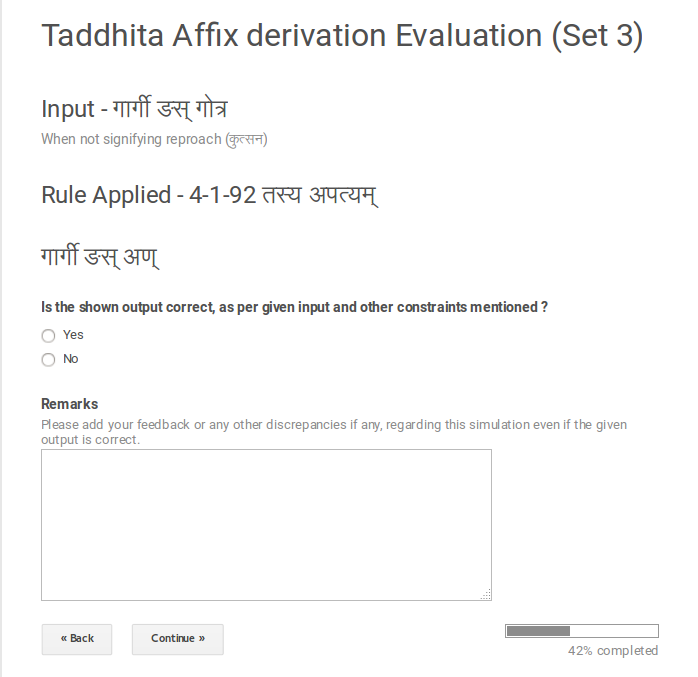
\includegraphics[width=0.8\textwidth]{evalPic}
    \caption{Snapshot of the evaluation framework}
    \label{evalFig}
\end{figure}

The results of the evaluation are shown in Table \ref{evalTab}. From among the 60 input cases, a total of ten cases were evaluated as being incorrect. As already discussed in Section \ref{sect:confRes}, the system has internalized vipratiṣedha as its default conflict resolution mechanism. The outputs were obtained with no other conflict resolution mechanism being employed. Ten cases resulted in wrong output. We later implemented the specificity hierarchy  for conflict resolution and then obtained the outputs again for the same set of input cases. This time, the number of incorrect output cases were reduced to 4. We will be discussing some of the wrong output cases in Section \ref{wrongCases}.  

\begin{table}[h]
\caption{Evaluation results for the experimental setup}
\label{evalTab}

\resizebox{0.9\textwidth}{!}{%
\begin{subtable}[t]{4in}
\caption{Details about the experimental setup}

\begin{tabular}{lc}
\hline
\multicolumn{1}{|l|}{Number of Input cases}                                                                                                  & \multicolumn{1}{c|}{60} \\ \hline
\multicolumn{1}{|l|}{Evaluators Participated}                                                                                                & \multicolumn{1}{c|}{5}  \\ \hline
\multicolumn{1}{|l|}{Inputs per evaluator}                                                                                                   & \multicolumn{1}{c|}{20} \\ \hline
\multicolumn{1}{|l|}{Numebr of Correct cases}                                                                                                & \multicolumn{1}{c|}{50} \\ \hline
\multicolumn{1}{|l|}{\begin{tabular}[c]{@{}l@{}}Number of Wrong output \\ (with no external conflict resolution)\end{tabular}}               & \multicolumn{1}{c|}{10} \\ \hline
\multicolumn{1}{|l|}{\begin{tabular}[c]{@{}l@{}}Number of wrong outputs\\ (with specificity hierarchy for conflict resolution)\end{tabular}} & \multicolumn{1}{c|}{4}  \\ \hline
                                                                                                                                             & \multicolumn{1}{l}{}   
\end{tabular}
\end{subtable}

\begin{subtable}[t]{3in}
\caption{Accuracy of the evaluation results}
\begin{tabular}{|l|c|c|}
\hline
Evaluation                           & \multicolumn{1}{l|}{Accuracy} & \multicolumn{1}{l|}{Error} \\ \hline
With no external conflict resolution & 83.33                         & 16.67                      \\ \hline
With specificity hierarchy           & 93.33                         & 6.67                       \\ \hline
\end{tabular}
	\end{subtable}

}
\end{table}


\begin{itemize}

\section{Analysis of Wrong Cases and Other Special Cases.}
\label{wrongCases}

\item For inputs {\skt उत्स ङस् अपत्यम्, दिति ङस् अपत्यम्}, the rules that got applied were \textsl{ A.4.1.95 and \sl A.4.1.122} respectively and those two rules essentially looks for phonological properties (ending sound, 	presence of vowel etc.). The correct rules to be applied for the instances are \textsl{ A.4.1.86 and A.4.1.85} respectively. Though those rules have same topical heads, they are specified before the current winner rules in Aṣṭādhyāyi, and hence by principle of vipratiṣedha  the former got preference over the desired ones. But if we observe they are more specific than the current winner rules. The correct rules have specificty at morphological level where specific stems are being mentioned, while the current winner rules have specificity at phonological level. Please note that  the mentioned rules carries entities that bear semantic specificity. But, since all the rules have that notion of semantic specificity, the effect from the notion is nullified here.

\item For inputs {\skt गर्ग ङस् गोत्र,  कपि ङस् गोत्र}, the rules that got applied are \textsl{ A.4.1.151 and A.4.1.122} instead of rules \textsl{ A.4.1.105 and A.4.1.107} respectively. Any rule in apatya section, or for that matter any rule under the 'arthādhikāra' has a semantic specificity by default, which is the semantic sense. But in this case, the rules \textsl{ A.4.1.105 and 107} are being mentioned in a granular level of semantic specificity of gotra, while the current applied rules deal the  general case of apatya. Please note that gotra is a specific sub-type of apatya. So whenever the intended semantic sense is gotra, and if there exists a rule that is applicable and has gotra specification, then it should be applied if conflicting with a rule of apatya specification.

\item For the input {\skt पितृष्वसृ ङस् अपत्यम्}, Ideally two output cases should appear, {\skt पितृष्वसृ ङस् छण्  and पितृष्वस् ङस् ढक्}. It is not rare in Taddhita derivation to see the applicability of multiple affixes for a single input case. But here the second output is the result of the rule \textsl{ A.4.1.133} {\skt ढकि लोपः}.The rule states that the final{\skt ऋ} in {\skt पितृष्वसृ} will be elided. Now no other rule mentions about affixation of {\skt ढक्} for the given input case. While implementing the rule \textsl{ A.4.1.133}, an assumption is made that the at first affix {\skt ढक्} should be introduced and then the elision operation should be performed. The basis of this assumption comes from the argument by many of the linguists that Pāṇini by specifying about the condition in \textsl{ A.4.1.133} implies that the affix {\skt ढक्} should be introduced \cite{rsbook}. It is argued that for the sake of brevity Pāṇini explicitly didn't mention the rule, but if the affixation is not implied then there is no purpose for the rule.\footnote{Our implementation has followed this assumption.}

\item In case of rule \textsl{ A.4.1.115 \skt मातुः उत् सङ्ख्यासम्भद्रपूर्वायाः}, here the stem mātṛ, will get its 'ṛ' replaced with 'u' provided if it satisfies the conditions given in the rule, by virtue of rule \textsl{ A.1.1.115}. Now when it comes to automation of such a step in derivation, it needs to be understood here that the operation is triggered immediately after affixation. This can be either seen as a continuum that is as the effect of the affixation rule itself or it can be seen as a separate rule triggering. The former doesn't adhere to Paninian way. So there should be some triggering mechanism which can handle rule triggering other than explicitly hardcoding rule triggering inside another rule. It would be ideal if a more elegant mechanism for triggering such rules can be employed. An elegant solution for such special cases are yet to be identified. Please note that triggering rules for identifying 'it' markers which is normally the next step or searching for a 'samña' rules are already implemented, but the case of triggering rules like \textsl{A.1.1.115} creates a hurdle in automation.

\item In case of rule \textsl{ A.4.1.122}, the rule is applicable specifically for nominals that has an 'i' as its last phonological entity but not by virtue of {\skt इञ्} affix attached to them. Such rules cannot be triggered unless and until one has prior knowledge about the affixes that the word-forms has from prior derivation. For such a purpose when automating, we should either keep a list of words beforehand, or else there should be some mechanism to store the extra information. Our system currently stores a list of some stems to tackle the issue as of now as we will be taking text inputs from the user. But what is more significant is that our 'śabdarūpa' object provides the functionality to store all those extra information like the it marker {\skt ञ्} which otherwise will not be present in the final word-form.

\end{itemize}


          


 
% Please add the following required packages to your document preamble:
% \usepackage{graphicx}


%%%%%%%%%%%%%%%%%%%%%%%%%%%%%%
%%End Of CHAPTER 5
%%%%%%%%%%%%%%%%%%%%%%%%%%%%%%%
\chapter{Discussion and Conclusion}
\lhead{Discussion and Conclusion}
\chaptermark{Discussion and Conclusion}
\label{chapter 6}

\section{The Schema as a General Schema for Modelling Aṣṭādhyāyī}
\label{sect:gen}

In section \ref{fig:fullImp}, we have seen the working of the system. In this section we will be discussing about the working of the sytem when we consider the rules that are outside of Taddhita section. \newcite{scharf10a} discusses five instances in which conflict of application occurs between two competing rules. In his paper, Scharf talks about conflict between rules \textsl{ A.6.1.87 } and \textsl{ A.6.1.88} where the domain of application of \textsl{ A.6.1.88} is properly contained within the domain of application of rule \textsl{ A.6.1.87}. Here \textsl{ A.6.1.88} should emerge as the winner rule, or else 6.1.88 will never be applied to any context. In our system \textsl{ A.6.1.87} is a direct descendant of \textsl{ A.6.1.84} which is a direct descendant of \textsl{ A.6.1.77}. The only aspect that is passed from \textsl{ A.6.1.77} as part of inheritance is {\skt अचि}, which is nothing but checking for a vowel as a right context. One might argue that \textsl{ A.6.1.84} does not have any relevance for this checking, but \textsl{ A.6.1.84} is an adhikāra rule and hence the execution will never stop at the rule, instead it will surely traverse down to one of the descendant rules. Also, its domain of influence is completely within the set of rules which is under the influence of rule \textsl{ A.6.1.77}. Now \textsl{ A.6.1.87} is one such rule. It is also evident from this instance as to how the rule is inheriting a set of mutually exclusive features and conditions by multilevel inheritance, avoiding the need for multiple inheritance. \textsl{ A.6.1.88} is also one such rule, but it needs an additional checking of condition which is checked also at \textsl{ A.6.1.87}. So in our system \textsl{ A.6.1.88} inherits from \textsl{ A.6.1.87} and becomes descendant of \textsl{ 6.1.87} by virtue of the anuvṛtti of {\skt आद्}. So whenever environment object is passed on to \textsl{ A.6.1.87}, it first checks presence of {\skt अ or आ} as the left context and then notifies all its registered rules including \textsl{ A.6.1.88}. If the rule is applicable to \textsl{ A.6.1.88}, i.e., if the environment satisfies all the conditions as demanded by \textsl{ 6.1.88} then it gets activated. So in addition to check for left context as per \textsl{ A.6.1.87}, \textsl{ A.6.1.88} also checks for {\skt एच्} as right context, which is applicable only to itself. This check is further restricting the scope of application to what occurred at rule \textsl{ A.6.1.77} where the checking was for {\skt अच्}.  This if evaluates to 'true' will block the direct application of \textsl{ A.6.1.87} i.e. guṇa will not happen there, but instead vṛddhi  will take place. If no rules turn out to be eligible for application, then only \textsl{ A.6.1.87} will perform the application of guṇa over the environment. Please note that the checking of other conditions that are applicable to these rules are not discussed here as those conditions are obtained by virtue of anuvṛtti and are being checked in the parent rules.
\\ \\
Now let us consider a case where partial blocking occurs when the rules \textsl{ A.6.1.77} and \textsl{ A.6.1.101} are in conflict. Our system deals with this in the same manner as we dealt with simple blocking. Rule \textsl{ A.6.1.101} inherits {\skt अचि}, i.e. element of \textsl{ ac} pratyāhāra, as right context. One thing to notice here is that the rule \textsl{ A.6.1.77} also checks for {\skt इकः}, i.e.,  element of \textsl{ ik} pratyāhāra in the context. But this is not carried forward as anuvṛtti. Now this rule is modeled as follows. The environment is passed onto \textsl{ A.6.1.77} and then it first checks for {\skt अचि}. Since only this is carried as anuvṛtti, once this condition evaluates to 'true', the rule notifies all rules registered with it. It waits for any of its descendants to claim eligibility. If no rule claims eligibility then the rule checks for additional condition of {\skt इकः} and if the condition evaluates to 'true', it claims the eligibility. In case of conflict between \textsl{ A.6.1.77} and \textsl{ A.6.1.101}, the desired rule is \textsl{ A.6.1.101}, but A.6.1.101 is a descendant of \textsl{ A.6.1.77}, so it will claim its eligibility and hence \textsl{ A.6.1.77} will be blocked from claiming its eligibility as per our system. From these examples it is evident that the system, without even using any extra conflict resolution techniques, can resolve the conflicts here. These examples demonstrate that the system internalizes rule \textsl{ A.1.4.2} {\skt विप्रतिषेधे परं कार्यम्}. Now consider the case when there is a conflict between the rules \textsl{ A.7.3.111} and \textsl{ A.7.1.73}.  Here both the rules belong to domain of aṅga, i.e., rule \textsl{ A.6.4.1}. Neither of the rules inherit from the other, and hence both of them are at sibling level and have a common parent at rule \textsl{ A.6.4.1}. In such a case where both the rules claim eligibility, the conflict which is at the level of rule \textsl{ A.6.4.1}, needs to be resolved. The desired rule in such a case is \textsl{ A.7.1.73}. The important point to be noted here is that though the system internalizes the concept of \textsl{ A.1.4.2}, it still does not claim \textsl{ A.7.3.111} as the winner rule. Instead the system will pass both the rules to the conflict resolution method coded as a separate function in the system, once it reaches the object for the rule \textsl{ A.6.4.1}.  

\\ \\
As discussed in Section \ref{sect:confRes}, we first implemented the four principles stated in 	'Nāgeśa's' 'pūrvaparanityāntaraṅgāpavaḍānāmuttarottaram balīyaḥ'. As expected for the cases which is discussed in the section \ref{sect:confRes} like \textsl{ A.6.1.77 vs.\sl A.3.4.86}
 and \textsl{ A.6.1.8 vs. A.6.1.77} and some other cases, we were able to resolve the conflicts and apply the desired rule. But for the case of conflict between rules \textsl{ A.7.1.73 and A.7.3.111} our system was still applying the rule \textsl{ 7.3.111} as per the priority for para, the rule which is stated later. But in this case, it is not the desired rule. The conflict occurs, when the input is a neuter stem which is 'i' or 'u' with an end marking of 'ṅ'. In \newcite{cardona65}, he discusses this particular rule conflict case. Cardona's work justified the selection of desired rule over the conflicting rule by stating the condition of presence of 'napuṃsaka'(neuter stems). This is a semantic feature, while the other rule does not have a semantic feature in its rule. Though he does not mention about the speicficity hierarchy but as a case of special case rule as in (general-exception case), it can be observed that this issue thus can be resolved by the specificity hierarchy of conflict resolution mechanism. 


Other conflicting instances discussed in \newcite{scharf10a} are not discussed here as those fall into any one of the scenarios already discussed.

\section{Bottlenecks in Automating the Astadhyayai}
\label{bottlenecks}

Our attempt was to automate the Taddhita section in Astadhyayai which primarily deals with affixation of derivational nouns. It is evident from the discussion so far, that Pāṇini uses a rich set of linguistic features in formulating rules and conditions to check for, before affixation. From the discussion about specificty hierearchy, we can see that the entire Aṣṭādhyāyi has used a variety of linguistic features ranging from phonetic to semantic features. Along with such features, Pāṇini sometimes has used intention of the speaker as a condition to be satisfied. For example, if we consider the rule \textsl{ 4-1-147 \skt गोत्रस्त्रियाः कुत्सने ण च }, the term {\skt कुत्सन} signifies 'reproach'. This is the intention of speaker whether to address someone by referring through the 'descendant of' relation in a disrespectful way or not. Such an aspect cannot be captured beforehand. So while implementing the automated system, we either had to generate all the alternatives, whenever the condition is to be satisfied is an intention, or else ask for human intervention to clarify the intention. We proceeded with the latter method as the former strictly doesn't adhere to the intended output derivation of the grammar. 
\\ \\ 
In Section \ref{wrongCases}, the first case can raise a question about our assumption in the specificity hierarchy. The desired rule for the instance discussed is \textsl{ A.4.1.86} and the conflicting rule is \textsl{ A.4.1.95}. Now if we look into the rule contents, we can find that rule \textsl{ A.4.1.86} does not come under any 'arthādhikāra', and only comes under a 'pratyayādhikāra' and \textsl{ A.4.1.95} has an 'arthādhikāra'. It can be argued that \textsl{ A.4.1.95} has a higher priority as per specificity hierarchy as it has a semantic condition, but the desired rule does not have a semantic condition, but only a morphological condition. Two observations motivated us for the existing assumption. The linguistically motivated counter argument is that if we go by the former argument, then the rule \textsl{ A.4.1.86} will never find its applicability. From the implementation aspect of view, the default affix rule \textsl{ A.4.1.83} and its exceptions which include \textsl{ A.4.1.86} as well, gets to apply the prefix after a suitable semantic relation is found, which are later rules like \textsl{ A.4.1.92}, which is in fact a semantic condition and this nullifies the effect. The assumption still needs to be validated in other similar rule conflict cases outside of Taddhita section.
\\ \\
In Section \ref{sect:gen}, we have talked in length about how the system has internalized the rule \textsl{ A.1.4.2}. Among different type of rules that Pāṇini formualted in his treatise like interpretive rules, operational rules, metarules etc., \textsl{ A.1.4.2} is a metarule, that describes about how other rules are to be interpreted. There are many other metarules in Aṣṭādhyāyi like \textsl{ A.1.1.66, A.1.1.49 }. In our system we have internalised those concepts and directly applied those in our implementation logic. So in our implementation the metarules are assumed to be known and the metarules are followed, but there is no explicit entity defined for the same. Now when automating further research is required about the need of meta-rules to be coded as separate entities, to have their presence stated explicitly.

\section{Conclusions and Future directions}
\label{sect:conc}
The proposed schema, which is primarily aimed at the automated generation of affixation for derivative nouns, or what is called as Taddhita section, adopts a completely object oriented approach in modeling the system. To the best of the authors' knowledge, the system is first of its kind that focuses specifically on modeling Taddhita section of Aṣṭādhyāyī. The system not only focuses on generation of correct forms but also in producing the correct sequence of rules applied for the derivation process. This approach doubles the system as a tool for pedagogy, where a learner can use the system to learn about the derivation process by trying out nominal of his choice, rather than restricting himself to a fixed set of textbook examples or a set of stored samples. As already discussed, the system facilitates in adopting and trying out various conflict resolution methods for rule selection, which can be programmed separately and then invoked from the system. As there is no consensus over one correct set of resolution methods, the proposed system can be used as a validation tool for verifying the accuracy of different conflict resolution methods that have been mentioned in various scholarly works. We have implemented some of the methods and those were discussed in Section \ref{sect:confRes}. In fact, we have not yet mentioned about one of the major areas of application for the proposed system. Since the system is essentially generating nouns (or adjectives) from other nouns (or adjectives) based on semantic relations, the system can be used to obtain relations between different nominals in an automated way. This kind of information can be used to supplement available lexical resources like IndoWordNet for sanskrit \cite{pushpak10} and also to provide supplementary information in dictionary entries for lexical databases as described in \newcite{huet2004design}.
\\ \\
Our system forms rule groups as Directed Acyclic Graphs (DAG), analogous to as \newcite{subbanna09} suggests. But our notion of topical rule groups  arises from the notion of topicality by virtue of anuvṛtti, while \newcite{subbanna09} attempts to form the topical rule groups from general-exception rule concepts. The approaches in group formation need to be studied further, in order to comment on the commonality of the DAGs so formed, but \newcite{subbanna09} do not talk about the attempts to model their concept in implementation. As each rule class implements precisely what is mentioned in the rule, and the implied portion is inherited by virtue of anuvṛtti from the parent class, the system can keep a trace of all the parent rules that have acted upon the environment, due to triggering of a particular rule. This gives the learner a much more detailed view of triggering of rules. The śabdarūpa object discussed in Section \ref{sect:woring} is also an object based implementation, environment mostly stores properties and does not have methods or functions that model any aspect of Aṣṭādhyāyī. The functions or methods implemented in śabdarūpa object are mostly for programmatic conveniences or adding functionality to the system front-end. This makes the set up of śabdarūpa object comparable to the set up as in \newcite{scharf14} which is primarily an XML representation. The conversion of objects to XML schema is a well addressed task in IT World \cite{jain2002xml}. Hence one can also think of developing a schema to transfer the data entities used in one system to the other, as \newcite{scharf14} tries to model the entire Aṣṭādhyāyī.  
\\ \\
With this thesis we were able to achieve the objectives set forth. From Chapter \ref{chapter 5} we can see how the system performs in an automated environment for the Taddhita section. The chapter also discusses the effect of conflict resolution methods we have implemented. The implementation details can be obtained in Chapter \ref{chapter 4}. The third objective was to implement a structure for storage of linguistic features that a particular word form should carry with it. Sections \ref{sect:intro-deri} and \ref{sect:egderi} discusses how the storage is performed along with the purpose of the same. We have also shown how affixation rules in Taddhita section tackles affix homonymy, synonymy etc. Though such a phenomena are not unique to sanskrit language, but it is ingenious to sanskrit that how Pāṇini tackles the issue by formulating the an inheritance network of rules and conditions within by utilizing a rich set of linguistic features which according to \newcite{deo07} is termed as constrained separationism.  




\clearpage
\titlespacing*{\chapter}{0pt}{-50pt}{40pt}
\chapter*{Bibliography}
\addcontentsline{toc}{chapter}{Bibliography}

\lhead{Bibliography}
\chaptermark{Bibliography}

\vspace{-50pt}
\begin{thebibliography}{50}
\lhead{Bibliography}

\bibliographystyle{acl}
\bibliography{myWork}



\end{thebibliography}
\cleardoublepage
% \phantomsection
\addcontentsline{toc}{chapter}{Appendix}

\begin{appendices}

\chapter {Publications from thesis}

Publications from the work presented in thesis:

\begingroup
\renewcommand{\chapter}[2]{}
\begin {thebibliography}{}
\bibitem[\protect\citename{Krishna and Goyal}2015]{krishna:15}
Amrith Krishna, Pawan Goyal.
\newblock 2015.
\newblock Towards automating the generation of derivative nouns in Sanskrit by simulating Pāṇini. 
\newblock In 16th World Sanskrit conference, Sanskrit and the IT world.
\end{thebibliography}
\endgroup

\end{appendices}


\end{document}